\documentclass{llncs}
\usepackage{amsmath}
\usepackage{llncsdoc}
\usepackage{amssymb} 
%\usepackage{amsthm}
\usepackage{ stmaryrd }
\usepackage{mathpartir}
%\usepackage{cite}
%\renewcommand{\citepunct}{,\,} % IEEEtran wants to use ],\,[ for this but that looks dumb...

\newcommand{\atlam}{@$\lambda$}

% Generic
\newcommand{\bindin}[2]{#1;~#2}
\newcommand{\pipe}{~\text{\large $\vert$}~}
\newcommand{\splat}[3]{#1_{#2};\ldots;#1_{#3}}
\newcommand{\splatC}[3]{#1_{#2}~~~~\cdots~~~~#1_{#3}}
\newcommand{\splatTwo}[4]{#1_{#3}#2_{#3},~\ldots~, #1_{#4}#2_{#4}}
\newcommand{\substn}[2]{[#1]#2}
\newcommand{\subst}[3]{\substn{#1/#2}{#3}}
\newcommand{\entails}[2]{#1 \vdash #2}

% Programs
\newcommand{\progsort}{\rho}
\newcommand{\pfam}[2]{\bindin{#1}{#2}}
\newcommand{\pdef}[4]{\bindin{{\sf def}~\tvar{#1}:#2=#3}{#4}}

% Families
\newcommand{\fvar}[1]{\textsc{#1}}

\newcommand{\family}[6]{{\sf family}~\fvar{#1}[#2]\sim \tvar{#5}.#6~\{#3\}}
\newcommand{\familyDf}{\family{Fam}{\kappaidx}{\opsort}{\opsigsort}{i}{\taurep}}

% Operators
\newcommand{\opsort}{\theta}
\newcommand{\opsigsort}{\Theta}
\newcommand{\opvar}[1]{\textbf{\textit{#1}}}

% Expressions
\newcommand{\evar}[1]{#1}
\newcommand{\elam}[3]{\lambda #1{:}#2.#3}
\newcommand{\eapp}[2]{{#1~#2}}
\newcommand{\eopapp}[2]{\eop{Arrow}{ap}{\tunit}{#1; #2}}
\newcommand{\eop}[4]{{\fvar{#1}.\opvar{#2}\langle#3\rangle(#4)}}
\newcommand{\elet}[4]{{\sf let}~#1 : #2 = #3~{\sf in}~#4}

% Type-Level Terms
\newcommand{\tvar}[1]{{\textbf{#1}}}

\newcommand{\tlam}[3]{\lambda \tvar{#1}{:}{#2}.#3}
\newcommand{\tapp}[2]{#1~#2}
\newcommand{\tifeq}[5]{{\sf if}~#1\equiv_{#3}#2{\sf ~then~}#4~{\sf else}~#5}
\newcommand{\tstr}[1]{\textit{``#1''}}
\newcommand{\tunit}{()}
\newcommand{\tpair}[2]{(#1, #2)}
\newcommand{\tfst}[1]{{\sf fst}(#1)}
\newcommand{\tsnd}[1]{{\sf snd}(#1)}
\newcommand{\tnil}[1]{[]_#1}
\newcommand{\tcons}[2]{#1 :: #2}
\newcommand{\tfold}[6]{{\sf fold}(#1; #2; \tvar{#3},\tvar{#4},\tvar{#5}.#6)}

\newcommand{\tfamSpec}[5]{{\sf family}~[#2]~::~#3~\{#4 : #5\}}
\newcommand{\tfamSpecStd}{\tfamSpec{fam}{\kappaidx}{\taurep}{\theta}{\Theta}}

\newcommand{\ttype}[2]{\fvar{#1}\langle#2\rangle}
\newcommand{\ttypestd}{\ttype{Fam}{\tau}}
\newcommand{\tfamcase}[5]{{\sf case}~#1~{\sf of}~\fvar{#2}\langle\tvar{#3}\rangle\Rightarrow#4~{\sf ow}~#5}
\newcommand{\trepof}[1]{{\sf rep}(#1)}

\newcommand{\tden}[2]{\llbracket #1~{\sf as}~#2 \rrbracket}
\newcommand{\ttypeof}[1]{{\sf typeof}~#1}
\newcommand{\tvalof}[2]{{\sf trans}(\tden{#1}{#2})}
\newcommand{\terr}{{\sf err}}
\newcommand{\tdencase}[5]{{\sf case}~#1~{\sf of}~\tden{\tvar{#2}}{\tvar{#3}}\Rightarrow#4~{\sf ow}~#5}

\newcommand{\titerm}[1]{\triangledown(#1)}
\newcommand{\titype}[1]{\blacktriangledown(#1)}

\newcommand{\tconst}[1]{{\sf const}(#1)}
\newcommand{\tOp}[1]{{\sf op}(#1)}

\newcommand{\tprog}[1]{{\sf program}(#1)}

\newcommand{\topsempty}{\cdot}
\newcommand{\tops}[5]{\opvar{#1}[#2](\tvar{#3},\tvar{#4}.#5)}
\newcommand{\topp}[2]{#1; #2}
\newcommand{\Tops}[2]{\tvar{#1} : #2}
\newcommand{\Topp}[2]{#1; #2}
\newcommand{\kOpEmpty}{\cdot}
\newcommand{\kOpS}[2]{\opvar{#1}[#2]}
\newcommand{\kOp}[3]{#1; \kOpS{#2}{#3}}

% Contexts
\newcommand{\fCtx}{\Sigma}
\newcommand{\itvarCtx}{\Omega}
\newcommand{\iCtx}{\Theta}
\newcommand{\eCtx}{\Gamma}
\newcommand{\etvarCtx}{\Omega}
\newcommand{\errCtx}{\mathcal{E}}
\newcommand{\famEvalCtx}{\Xi}

% Judgments
\newcommand{\emptyctx}{\emptyset}
\newcommand{\tvarCtx}{\Delta}
\newcommand{\tvarCtxX}[2]{\Delta, {\tvar{#1}} : {#2}}
\newcommand{\fvarCtx}{\Sigma}
\newcommand{\fvarCtxX}{\Sigma, \fvarOfType{Fam}{\kappaidx}{\Theta}}
\newcommand{\eivarCtx}{\Omega}
\newcommand{\eivarCtxX}[1]{\Omega, \evar{#1}}

\newcommand{\kEntails}[3]{#1 \vdash_{#2} #3}

\newcommand{\progProg}[1]{#1~{\tt prog}}
\newcommand{\progOK}[3]{\kEntails{#1}{#2}{\progProg{#3}}}
\newcommand{\progOKX}[1]{\progOK{\tvarCtx}{\fvarCtx}{#1}}

\newcommand{\fvarOfType}[3]{\fvar{#1}[#2,#3]}
\newcommand{\fvarOfTypeDf}{\fvarOfType{Fam}{\kappaidx}{\Theta}}

\newcommand{\opOfType}[2]{#1 : #2}
\newcommand{\opType}[4]{\kEntails{#1}{#2}{\opOfType{#3}{#4}}}

\newcommand{\tOfKind}[2]{#1 : #2}
\newcommand{\tKind}[4]{\kEntails{#1}{#2}{\tOfKind{#3}{#4}}}
\newcommand{\tKindX}[2]{\tKind{\tvarCtx}{\fvarCtx}{#1}{#2}}

\newcommand{\isExpr}[1]{#1~\texttt{expr}}
\newcommand{\exprOK}[4]{#1~#2 \vdash_{#3} \isExpr{#4}}
\newcommand{\exprOKX}[1]{\exprOK{\tvarCtx}{\eivarCtx}{\fvarCtx}{#1}}

\newcommand{\isIterm}[4]{#1~#2 \vdash_{#3} #4~\texttt{iterm}}
\newcommand{\isItermX}[1]{\isIterm{\tvarCtx}{\eivarCtx}{\fvarCtx}{#1}}

\newcommand{\isItype}[3]{#1 \vdash_{#2} #3~\texttt{itype}}
\newcommand{\isItypeX}[1]{\isItype{\tvarCtx}{\fvarCtx}{#1}}

\newcommand{\tEvalX}[2]{#1 \Downarrow #2}
\newcommand{\tiEvalX}[2]{#1 \curlyveedownarrow #2}

\newcommand{\fvalCtx}{\Phi}
\newcommand{\fvalCtxX}[1]{\Phi, #1}
\newcommand{\fval}[4]{\fvar{#1}[#2, \tvar{#3}.#4]}
\newcommand{\fvalDf}{\fval{Fam}{\theta}{i}{\tau}}

\newcommand{\pcompiles}[3]{\vdash_{#1} #2 \Longrightarrow #3}
\newcommand{\pcompilesX}[1]{\pcompiles{\fvalCtx}{#1}{\gamma}}

\newcommand{\ptcc}[2]{#1 \longrightarrow #2}

\newcommand{\etCtx}{\Gamma}
\newcommand{\etCtxX}[2]{\etCtx, \evar{#1} : #2}

\newcommand{\gtCtx}{\Psi}
\newcommand{\gtCtxX}[2]{\gtCtx, \evar{#1} : #2}

\newcommand{\ecompiles}[5]{#1 \vdash_{#2} #3 : #4 \Longrightarrow #5}
\newcommand{\ecompilesX}[3]{\ecompiles{\etCtx}{\fvalCtx}{#1}{#2}{#3}}

\newcommand{\delfromtau}[4]{\vdash^{\fvar{#1}}_{#2} #3 \sim #4}
\newcommand{\tauisdel}[5]{\vdash^{\fvar{#1}}_{#2} \ttype{#3}{#4} \sim #5}

\newcommand{\checkRC}[5]{#1 \vdash^{\fvar{#2}}_{#3} #4 \sim #5}
\newcommand{\checkRCX}[2]{\checkRC{\gtCtx}{Fam}{\fvalCtx}{#1}{#2}}

\newcommand{\erase}[3]{\vdash_{#1} #2 \leadsto #3}
\newcommand{\eraseX}[2]{\erase{\fvalCtx}{#1}{#2}}

\newcommand{\eCtxTogCtx}[4]{\vdash^{\fvar{#1}}_{#2} #3 \sim #4}
\newcommand{\eCtxTogCtxX}[2]{\eCtxTogCtx{Fam}{\fvalCtx}{#1}{#2}}

\newcommand{\ddbar}[4]{\vdash^{\fvar{#1}}_{#2} #3 \sim #4}
\newcommand{\ddbarX}[2]{\ddbar{Fam}{\fvalCtx}{#1}{#2}}

\newcommand{\iType}[3]{#1 \vdash #2 : #3}

\newcommand{\gtCtxH}{\hat{\gtCtx}}
\newcommand{\gtCtxHX}[2]{\gtCtxH, \evar{#1} : #2}

%
\newcommand{\fSpec}[3]{\tof{\fvar{#1}}{\kFam{#2}{#3}}}
\newcommand{\fSpecStd}{\fSpec{fam}{\kappaidx}{\Theta}}

% \tau
\newcommand{\taut}[1]{{\tau_{\text{#1}}}}
\newcommand{\tautype}{\taut{type}}
\newcommand{\tautrans}{\taut{trans}}
\newcommand{\tauproof}{\taut{proof}}
\newcommand{\tauidx}{\taut{idx}}
\newcommand{\taui}{\taut{i}}
\newcommand{\tauidxn}[1]{\taut{idx,#1}}
\newcommand{\taurep}{\taut{rep}}
\newcommand{\taurepn}[1]{\taut{rep,#1}}
\newcommand{\tauden}{\taut{den}}
\newcommand{\tauIT}{\taut{IT}}
\newcommand{\tauarrow}{\taut{arrow}}
\newcommand{\tauprod}{\taut{prod}}
\newcommand{\tauint}{\taut{int}}
\newcommand{\taubool}{\taut{bool}}
\newcommand{\tauprog}{\taut{prog}}
\newcommand{\tauiterm}{\taut{iterm}}
\newcommand{\tauval}{\taut{val}}
\newcommand{\tauop}{\taut{op}}

% \gamma
\newcommand{\ghat}{\hat{\gamma}}

% \sigma
\newcommand{\delt}[1]{\sigma_{\text{#1}}}
\newcommand{\delrep}{\delt{rep}}
\newcommand{\dhat}{\hat{\sigma}}
\newcommand{\dbar}{\bar{\sigma}}

% \kappa
\newcommand{\kappat}[1]{\kappa_{\text{#1}}}
\newcommand{\kappaidx}{\kappat{idx}}
\newcommand{\kappai}{\kappat{i}}

% Types

% IL terms
\newcommand{\ivar}[1]{\textrm{#1}}
\newcommand{\ilam}[3]{\lambda #1{:}#2.#3}
\newcommand{\ifix}[3]{{\sf fix~}#1{:}#2~{\sf is}~#3}
\newcommand{\iapp}[2]{#1~#2}
\newcommand{\ipair}[2]{(#1, #2)}
\newcommand{\ifst}[1]{{\sf fst}(#1)}
\newcommand{\isnd}[1]{{\sf snd}(#1)}
\newcommand{\iintlit}{\bar{
\textrm{z}}}
\newcommand{\iop}[2]{#1 \oplus #2}
\newcommand{\iIfEq}[5]{{\sf if}~#1\equiv_{#3}#2{\sf ~then~}#4~{\sf else}~#5}
\newcommand{\mvalof}[1]{{\sf valof}(#1)}
\newcommand{\iup}[1]{\vartriangle\hspace{-2.5pt}(#1)}

% Internal Types
\newcommand{\darrow}[2]{#1\rightarrow#2}
\newcommand{\dint}{\mathbb{Z}}
\newcommand{\dpair}[2]{#1\times#2}
\newcommand{\dup}[1]{\blacktriangle(#1)}
\newcommand{\drepof}[1]{{\sf repof}(#1)}

% Kinds
\newcommand{\kvar}[1]{\textrm{#1}}
\newcommand{\karrow}[2]{#1\rightarrow{#2}}
\newcommand{\kforall}[2]{\forall \kvar{#1}.#2}
\newcommand{\kstr}{\textsf{Str}}
\newcommand{\kunit}{\textsf{1}}
\newcommand{\kpair}[2]{#1 \times #2}
\newcommand{\klist}[1]{\textsf{list}[#1]}
\newcommand{\kTypeBlur}{\star}
\newcommand{\kDen}{\textsf{Den}}
\newcommand{\kIType}{\textsf{ITy}}
\newcommand{\kITerm}{\textsf{ITm}}

% Judgements
\newcommand{\tof}[2]{#1 : #2}
\newcommand{\mtof}[2]{#1 :: #2}
\newcommand{\tentails}[2]{#1 \vdash #2}
\newcommand{\tentailst}[3]{\tentails{#1}{\tof{#2}{#3}}}
\newcommand{\tStdCtx}{\fCtx~\tvarCtx}
\newcommand{\tCtxXF}[1]{\fCtx, #1~\tvarCtx}
\newcommand{\tCtxXT}[1]{\fCtx~\tvarCtx, #1}
%\newcommand{\tCtxXL}[1]{\fCtx~\tvarCtx~\lvarCtx, #1}
\newcommand{\tentailsX}[1]{\tentails{\tStdCtx}{#1}}
\newcommand{\tentailsXt}[2]{\tentailsX{\tof{#1}{#2}}}
\newcommand{\kentails}[2]{#1 \vdash #2}
\newcommand{\kentailsX}[1]{\kentails{\fCtx}{#1}}
\newcommand{\iMkCtx}[3]{#1~#2~#3}
\newcommand{\iStdCtx}{\iMkCtx{\fCtx}{\tvarCtx}{\itvarCtx}}
\newcommand{\ientails}[2]{#1 \vdash #2}
\newcommand{\ientailsX}[1]{\entails{\iStdCtx}{#1}}
\newcommand{\casemap}[2]{#1 : #2}
\newcommand{\mentails}[3]{#1, #2 \vdash #3}
\newcommand{\mentailsX}[1]{\mentails{\tvarCtx}{\itvarCtx}{#1}}
\newcommand{\eentails}[4]{#1~#2~#3 \vdash #4}
\newcommand{\eentailsX}[1]{\eentails{\fCtx}{\tvarCtx}{\etvarCtx}{#1}}
\newcommand{\mtentails}[2]{#1 \vdash #2}
\newcommand{\mtentailsX}[1]{\mtentails{\iCtx}{#1}}
\newcommand{\mtentailsXt}[2]{\mtentails{\iCtx}{\mtof{#1}{#2}}}
\newcommand{\kSimple}[1]{#1~{\sf simple}}
\newcommand{\Tentails}[3]{#1 \vdash_{#2} #3}
\newcommand{\TentailsX}[1]{\Tentails{\fCtx}{\fvar{fam}}{#1}}
\newcommand{\kEq}[1]{#1~\texttt{eq}}

% Verification and Translation
\newcommand{\translates}[4]{\entails{#1}{#2 \longrightarrow \tden{#3}{#4}}}

% Compilation Semantics
\newcommand{\compiless}[3]{#1 \Longrightarrow \tden{#2}{#3}}
\newcommand{\compiles}[3]{#1 \Longrightarrow \tden{#2}{#3}}
%\newcommand{\translates}[6]{\entails{#1}{\translatesTo{#2}{#3}{#4}{#5}{#6}}}
\newcommand{\translatesTo}[5]{#1 \longrightarrow \tden{#2}{\ttype{#3}{#4}{#5}{6}{7}}}
\newcommand{\translatesX}[5]{\translates{\eCtx}{#1}{#2}{#3}{#4}{#5}}


\renewcommand{\ttdefault}{txtt}
\usepackage{alltt}
\usepackage{listings}
\lstset{language=ML,
showstringspaces=false,
basicstyle=\ttfamily\footnotesize,
morekeywords={newcase,extends}}

\usepackage{float}
\floatstyle{ruled}
\newfloat{codelisting}{tp}{lop}
\floatname{codelisting}{Listing}

\usepackage{url}
% url.sty was written by Donald Arseneau. It provides better support for
% handling and breaking URLs. url.sty is already installed on most LaTeX
% systems. The latest version can be obtained at:
% http://www.ctan.org/tex-archive/macros/latex/contrib/misc/
% Read the url.sty source comments for usage information. Basically,
% \url{my_url_here}.

\usepackage{placeins}

%\lefthyphenmin=4
\hyphenation{op-tical net-works semi-conduc-tor}

\usepackage{todonotes}

\begin{document}
\mainmatter  % start of an individual contribution

% first the title is needed
\title{Active Typechecking and Translation: A Safe Language-Internal Extension Mechanism}

% a short form should be given in case it is too long for the running head
\titlerunning{Lecture Notes in Computer Science: Authors' Instructions}

% the name(s) of the author(s) follow(s) next
%
% NB: Chinese authors should write their first names(s) in front of
% their surnames. This ensures that the names appear correctly in
% the running heads and the author index.
%
\author{Cyrus Omar%
\and Jonathan Aldrich}
%
\authorrunning{Lecture Notes in Computer Science: Authors' Instructions}
% (feature abused for this document to repeat the title also on left hand pages)

% the affiliations are given next; don't give your e-mail address
% unless you accept that it will be published
\institute{Carnegie Mellon University, Pittsburgh, PA 15213, USA\\
\texttt{\{comar,aldrich\}@cs.cmu.edu}
}

%
% NB: a more complex sample for affiliations and the mapping to the
% corresponding authors can be found in the file "llncs.dem"
% (search for the string "\mainmatter" where a contribution starts).
% "llncs.dem" accompanies the document class "llncs.cls".
%

\toctitle{Lecture Notes in Computer Science}
\tocauthor{Authors' Instructions}
\maketitle


\begin{abstract}
Researchers and domain experts often propose new language primitives as extensions to the semantics of an existing language. 
But today's statically-typed languages are {monolithic}: they do not expose language-internal mechanisms for implementing the static and dynamic semantics of new primitive types and their associated operators directly, so these experts must instead create new standalone languages.
This causes problems for potential users because building applications from components written in many different languages can be both unsafe and unnatural. 
An {internally-extensible} language could  address these issues, but designing a mechanism that is expressive while maintaining safety remains a challenge. 
Extensions must be modularly verified, their use in any combination must not weaken the metatheoretic properties of the language, nor can they interfere with one another.
We introduce a mechanism called active type-checking and translation (AT\&T) that aims to directly address these issues while remaining highly expressive. 
AT\&T leverages type-level computation, typed compilation techniques and a form of type abstraction to enable library-based implementations of a variety of primitives over a flexible  grammar in a safe manner. 
%In a language supporting AT\&T, primitive types families are represented uniformly at the type level. Each type is equipped with operators, defined using type-level functions, that are invoked specifically during the type-checking and translation of operations relevant to that type. 
%We discuss three points in the design space: (1) a simple judgmental construction of AT\&T designed to distill the essential concepts and admit formal safety theorems, (2) a "real" language called Ace that we use to demonstrate the expressive power of AT\&T in practice, and (3) a language design called Birdie that lifts and extends CoqÍs rich system of dependent types into the type-level, allowing extension developers to fully prove the correctness of extensions statically.
\keywords{extensible languages; active libraries; typed compilation; type-level computation; type abstraction}
\end{abstract}

\section{Motivation}
When designing and implementing a new abstraction, experts typically begin by attempting to define new constructs in terms of existing language constructs.
This approach is often effective because modern {general-purpose} abstraction mechanisms, like inductive datatypes and object systems, are highly expressive.  
For example, the Delite framework leverages Scala's powerful general-purpose mechanisms to enable a number of useful \emph{embedded domain-specific languages} \cite{delite}.
Unfortunately, there remain some situations of interest where general-purpose abstractions fall short. 
For instance, it is difficult to adequately encode advanced type systems in terms of the simpler rules that govern general-purpose abstractions (e.g. reasoning about units of measure requires built-in language support in F\# \cite{conf/cefp/Kennedy09}). 
Even if a full encoding is possible, it may not be useful if it is overly verbose or unnatural, or if the error messages are overly abstract. For example, regular expressions encoded using inductive datatypes are quite verbose, so most functional languages support them via strings, which is less safe. 
Finally, general-purpose abstractions are implemented in a uniform manner, meaning domain-specific heuristics cannot be applied to eliminate overhead or perform optimizations, and implementations designed for typical application workloads may not be satisfactory in parts of a program where performance is a key criteria, such as when targeting heterogeneous hardware platforms (e.g. programmable GPUs) and distributed computing resources.

% are at times impossible or impractical. In our example of adding products or sums to Godel's T, although Church encodings are possible \cite{pfpl}, they require a reasonable level of creativity\footnote{Anecdotally, Church encodings are among the more difficult-to-explain topics covered in our undergraduate programming languages course.}. Moreover, they will not offer the same static safety guarantees as a primitive encoding, they are more verbose and they will incur performance overhead by their use of closures rather than a more direct representation. This is not only a problem for simple languages like Godel's T. Several Haskell-based embedded DSLs have also needed to make significant compromises at times \cite{haskellDSLs}. {\color{red} examples? Scala?}

%creating a new language. If this is not practical, the best one can attempt to do is encode the new types in terms of existing types (by a Church encoding, for example). This is generally unsatisfactory -- 

%Languages implemented using these common patterns are central planning by a language designer or design committee. 

Researchers or domain experts who run into situations like these, where more direct control over a language's semantics and implementation are needed, have little choice today but to realize new abstractions by creating a new language in some way. They might develop a new standalone language from scratch, modify an implementation of an existing language, or use tools like compiler generators, DSL frameworks and language workbenches \cite{fowler2010domain}. 
%In our simple scenario, we may simply fork our implementation of Godel's T or even edit it directly (a pernicious technique for implementing a new language where the prior one is overwritten). 
%In a more complex scenario, we may instead employ a tool like a compiler generator or DSL framework \cite{fowler2010domain} that can generate a standalone implementation from declarative specifications of language constructs. Some of these tools allow you to package and reuse these specifications (with the important caveat that not all combinations of constructs are valid and free of conflicts, an important modularity issue that we will return to several times in this paper).
The increasing sophistication and ease-of-use of these tools have led to calls for a {\it language-oriented approach} to software development, where different components of an application are written in different specialized languages \cite{journals/stp/Ward94}. Indeed, a number of software ecosystems are now designed explicitly to support many different languages, both general-purpose and domain-specific, atop a common intermediate language. The Java virtual machine (JVM), the Common Language Infrastructure (CLI) and LLVM are prominent examples of such ecosystems.

Unfortunately, this leads to a critical problem at language boundaries: a library's external interface must only use constructs that can reasonably be expressed in \emph{all possible client languages}. This discourages languages from including constructs that rely on statically-checked invariants stronger than those supported by their underlying implementation in the common intermediate language. At best, constructs like these can be exposed by generating a wrapper where run-time checks have been inserted to guarantee these invariants. This compromises both verifiability and performance. %Forrequires the development of an interoperability layer for every pair of DSLs. 
Moreover, this approach exposes the internals of an implementation to clients, making the abstraction awkward to work with and causing code breakage when implementation details change. This defeats a primary purpose of high-level programming languages: hiding low-level details from clients of an abstraction. We diagram this fundamental \emph{interoperability problem} in Figure \ref{approaches}(a). 
%As an example, F\#'s type system prevents \lstinline{null} values from occurring within data structures, but because it's type system is not available when calling into F\# code from another language, like C\#, run-time null checks must still be included in the implementation.
\begin{figure}[t]
\vspace{-15px}
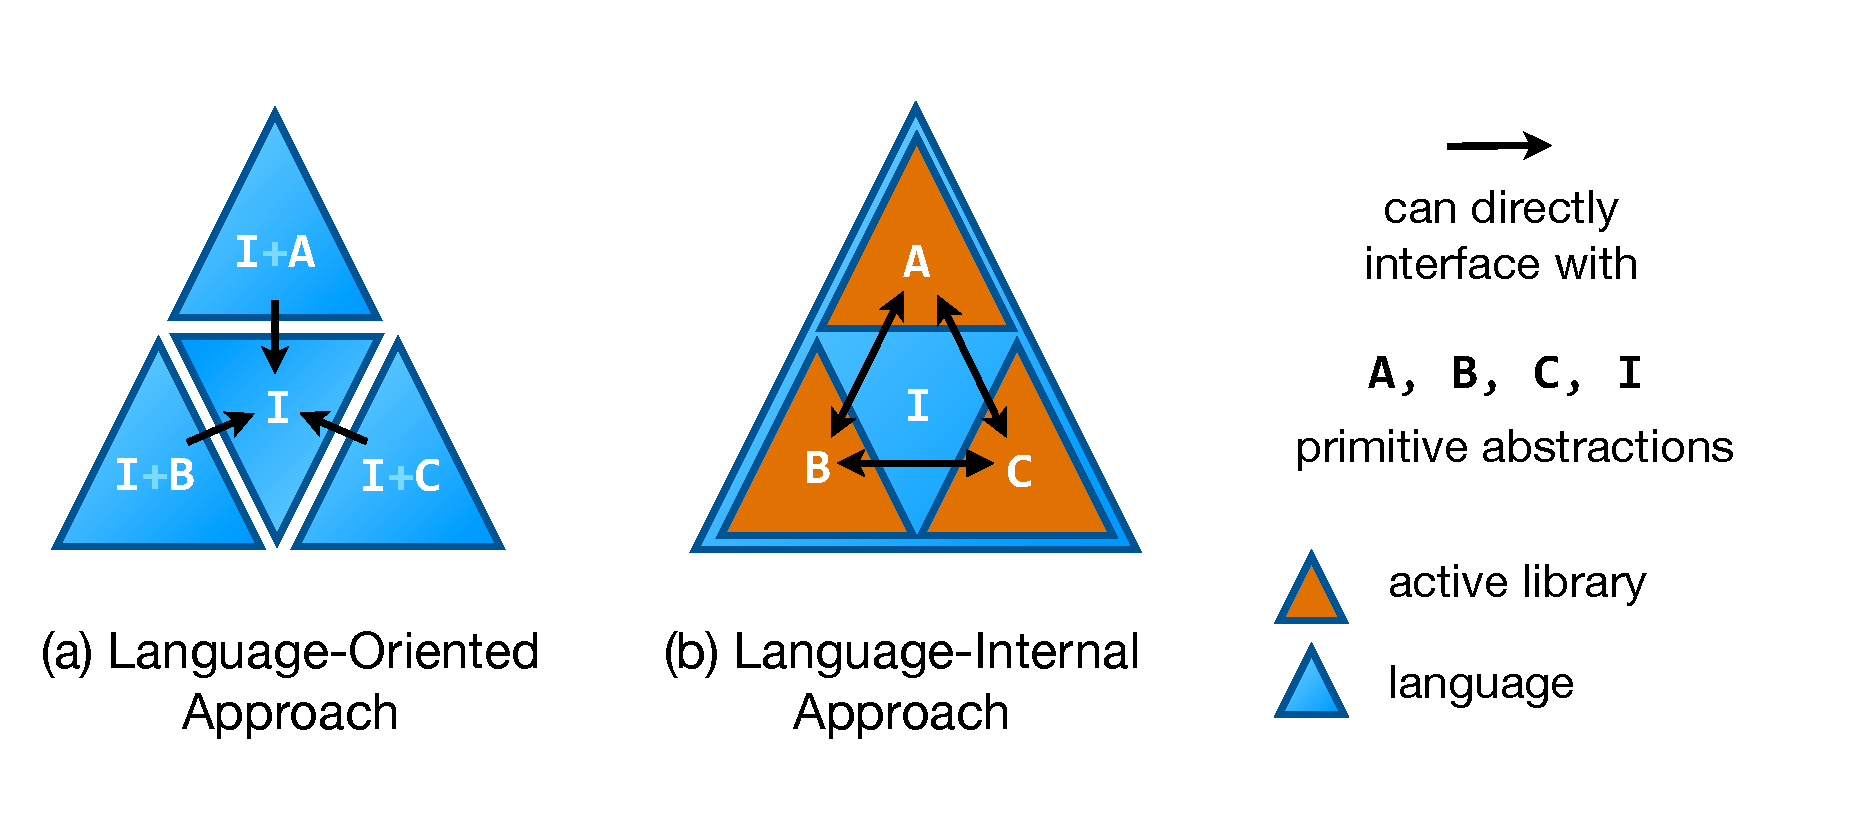
\includegraphics[scale=0.415]{approaches.pdf}
\vspace{-30px}
\caption{(a) With the language-oriented approach, different primitive abstractions are packaged into separate languages that extend and target a common intermediate language (e.g. JVM bytecode). Users can only interface with libraries written in another language via the constructs in the common language, causing \emph{interoperability problems}. (b) With the language-internal approach, the semantics of new abstractions (i.e. the logic that governs typechecking and translation to a fixed {internal language}, here labeled \texttt{I}) can be implemented directly within so-called \emph{active libraries}. Clients can import and use these abstractions directly whenever needed.}
\vspace{-10px}
\label{approaches}
\end{figure}

%As a result, domain-specific languages and new general-purpose abstractions alike have experienced relatively slow adoption in practice.
%
%Porting large codebases to new languages is difficult, and the dominant programming languages innovate slowly, so programming language.
%
%More specifically, such languages are neither \emph{internally extensible} because the language itself exposes only natural numbers and functions to its users, nor are they \emph{externally extensible} because no new behaviors can be added to the language's  implementation in a separate module from the one containing the initial implementation.

%This is the essence of a monolithic language implementation: it is impossible for anyone to modularly extend languages defined in this way. 

%Programming languages are typically designed around a monolithic collection of primitive type families and operators. Consider, as a simple example, Godel's T \cite{pfpl}, a typed lambda calculus with recursion on primitive natural numbers\todo{add statics to Appendix A}. Although a language designer may casually speak of ``extending Godel's T with primitive product and sum types'', adding these type families and associated operators to this kind of language from within is impossible. That is, Godel's T is not \emph{internally extensible}.

\emph{Internally-extensible programming languages} promise to avoid these problems by providing researchers and domain experts with a mechanism for implementing the semantics of new primitive constructs directly within libraries.
%Developers of libraries need only determine whether they are appropriate for their domain, without also considering whether these constructs can be exposed in terms of abstractions appropriate to client code. 
As a result, clients can granularly import any necessary primitive constructs when using code that relies on them, and thereby achieve full safety, ease-of-use and performance. Providers of components thus need only consider whether primitives that they use are appropriate for their domain, without also considering whether their code might be used in a context where these primitives are not otherwise appropriate. Libraries containing logic that is invoked at compile-time, as extension logic would be, have been called \emph{active libraries} \cite{activelibraries}. We adopt this terminology and diagram this competing approach in Figure \ref{approaches}(b).

%Researchers and domain experts thus gain the ability to distribute new ideas for evaluation to a broader development community without requiring the approval of maintainers of mainstream languages, large-scale porting of code or explicit interoperability layers. 

For a language-internal extension mechanism to be feasible, however, it must achieve expressiveness while also ensuring that extensions cannot compromise the safety properties of the language and its tools, nor interfere with one another. That is, extensions cannot simply be permitted to add arbitrary logic to the type system or compiler, because this would make it possible to break  type safety, decidability or adequacy theorems that are critical to the operation of the language, the compiler or other extensions. We review some previous attempts at language extensibility, and highlight how they do not adequately achieve both safety and expressiveness, in Section \ref{related-work}.
%{\color{red} transition here} Correctness properties of an extension itself should be modularly verifiable, so that its users can rely on it for verifying and compiling their own code. The mechanism must also ensure that desirable metatheoretic properties and global safety guarantees of the language cannot be weakened by extensions. And with multiple independently-developed extensions used at once, the mechanism must further guarantee that they cannot interfere with one another. 

In this paper, we introduce a language-internal extensibility mechanism called \emph{active typechecking and translation} (AT\&T) that allows developers to introduce and implement the logic governing new primitive type and operator families from within libraries. 
We argue that this can be accomplished by enriching the type-level language, rather than introducing a separate metalanguage into the system. 
To make this proposal concrete, we begin by introducing a simple core calculus, called \atlam~(for the ``actively-typed lambda calculus''), in Section \ref{atlam}. 
This calculus uses type-level computation of higher kind, along with techniques borrowed from the typed compilation literature and a form of type abstraction that ensures that the implementation details of an extension are not externally visible to guarantee the safety of the language, the decidability of typechecking and compilation and non-interference of extensions, as we outline in Section \ref{safety}.
In Section \ref{examples}, we suggest that despite these constraints, this mechanism is expressive enough to admit, within libraries, a number of general-purpose and domain-specific abstractions that normally require built-in language support. 

%Our core calculus uses a uniform abstract syntax for primitive operators to simplify our presentation and analysis, but this syntax is too verbose to be practical. Thus, we begin this section by showing how a key design choice made in the calculus -- to associate operators with type families, forming what we call \emph{active type families} -- supports a novel type-directed desugaring mechanism that permits the use of conventional concrete syntax for language extensions. 

% Our choice of a simply-typed, simply-kinded calculus where expressions are given meaning by translation to a simply-typed internal language appears to occupy a ``sweet spot'' in the design space, and relates closely to how simply-typed functional languages like  ML and Haskell are specified and implemented today. In Section \ref{design}, we briefly discuss other points in the design space of actively-typed languages and describe the sorts of abstractions that the mechanism as we have introduced it is not capable of expressing, suggesting several directions for future research. We conclude with a discussion of related work in Section \ref{related-work}.
%dependently-typed and object-oriented type-level languages, as well as the constraints governing the design of the internal language.  
%We will also note how object-oriented techniques may also be suit, because of a fundamental connection to the \emph{expression problem} \cite{expression-problem}.

%specify new typechecking rules and translation logic from within libraries. The AT\&T mechanism utilizes type-level computation of higher kind and integrates typed compilation techniques into the language to provide strong safety guarantees, while remaining straightforward and expressive.

%AT\&T is general with respect to many choices about the type-level language, the typed internal language and syntax. Choices along these dimensions can affect both expressiveness and ease-of-use. We will begin in Sec. 2 by introducing a minimal system called $@\lambda$ (the ``actively-typed lambda calculus'') that distills the essence of the mechanism in a simply-typed, simply-kinded setting. This will allow us to fully and concisely formalize the language and compiler and give several key safety theorems. We will then continue in Sec. 3 by discussing variants of this mechanism based on other basic paradigms, considering dependently-typed functional languages and object-oriented languages, discussing trade-offs between expressivity and safety when doing so. We have developed a simple prototype called Ace and have used it to develop a number of full-scale language extensions as libraries. We will briefly discuss this language and these extensions in Sec. 4.

%We note at the outset that AT\&T focuses on extending the static semantics of languages with fixed, though flexible, syntax. Language-internal syntax extension mechanisms have been developed in the past (e.g. SugarJ \cite{sugarj}) but they have also suffered from safety problems because grammar composition is not always safe when done in an  unconstrained manner. Constrained approaches that provide stronger safety guarantees have recently been outlined (e.g. Wyvern \cite{globaldsl13}) but we will leave integration of syntax extensions with semantic extensions as future work.
\section{From Extensible Compilers to Extensible Languages}\label{evolution}
To understand the genesis of our internal extension mechanism, it is helpful to begin by considering why most implementations of programming languages cannot even be  externally extended. 
Let us consider, as a simple example, an implementation of G\"odel's T, a typed lambda calculus with recursion on primitive natural numbers (see Appendix). 
A compiler for this language written using a functional language will invariably represent the primitive type families and operators using {closed} inductive datatypes. 
For example, a simple implementation in Standard ML may be based around these datatypes:
\begin{lstlisting}
  datatype Type = Nat | Arrow of Type * Type
  datatype Exp = Var of var 
               | Lam of var * Type * Exp | Ap of Exp * Exp 
               | Z | S of Exp | Natrec of Exp * Exp * Exp
\end{lstlisting}

The logic governing typechecking and translation to a suitable intermediate language (for subsequent optimization and compilation by some back-end) will proceed by exhaustive case analysis over the constructors of \lstinline{Exp}.

In an object-oriented implementation of Godel's T, we might instead encode types and operators as subclasses of abstract classes \lstinline{Type} and \lstinline{Exp}. Typechecking and translation will proceed by the ubiquitous \emph{visitor pattern}  by dispatching against a fixed collection of {known} subclasses of \lstinline{Exp}. 

In either case, we encounter the same basic issue: there is no way to modularly add new primitive type families and operators and implement their associated typechecking and translation logic. 
%This issue is related to the widely-discussed \emph{expression problem} (in a restricted sense -- we do not consider adding new functions beyond typechecking and translation here, only adding logic to these) \cite{wadler-expression}.

A number of language mechanisms have been proposed that allow new cases to be added to datatypes and the functions that operate over them in a modular manner. 
In functional languages, we might use \emph{open datatypes}. For example, if we wish to extend G\"odel's T with product types and we have written our compiler in a language supporting open inductive datatypes, it might be possible to add new cases like this: 
\begin{lstlisting}
  newcase Prod of Type * Type extends Type
  newcase Pair of Exp * Exp extends Exp    (* Intro *)
  newcase PrL of Exp extends Exp           (* Elim Left *)
  newcase PrR of Exp extends Exp           (* Elim Right *)
\end{lstlisting}

The logic for functionality like typechecking and translation could then be implemented for only these new cases. For example, the \lstinline{typeof} function that assigns a type to an expression could be extended like so:
\begin{lstlisting}
  typeof PrL(e) = case typeof e of 
      Prod(t1, _) => t1 
    | _ => raise TypeError("<appropriate error message>")
\end{lstlisting}

If we allowed users to define new modules containing definitions like these and link them into our compiler, we will have succeeded in creating an externally-extensible compiler, albeit one where safety is not guaranteed (we will return to this point shortly). We have not, however, created an extensible programming language, for two reasons. First, compiler extensions are distributed and activated separately from libraries, so dependencies become more difficult to manage. Second, other compilers for the same language will not necessarily support the same extensions. 
If our newly-introduced constructs are exposed at a library's  interface boundary, clients using different compilers face the same problems with interoperability that those using different languages face. That is, {extending a language by extending a single compiler for it is morally equivalent to creating a new language}. Several prominent language ecosystems today are in a state where a prominent compiler has introduced or enabled the introduction of extensions that many libraries have come to rely on, including the Glasgow Haskell Compiler, SML/NJ and the GNU compilers for C and C++.

A more appropriate and useful place for extensions like this is directly within libraries, alongside abstractions that can be adequately implemented in terms of existing primitive abstractions. To enable this, the language must allow for the introduction new primitive type families, like \lstinline{Prod}, operators, like \lstinline{Pair}, \lstinline{PrL} and \lstinline{PrR}, and associated typechecking and translation logic. When encountering these new operators in expressions, the compiler must effectively  hand control over typechecking and translation to the appropriate user-defined logic. Because this mechanism is {language-internal}, all compilers must support it to satisfy the language specification.

Statically-typed languages typically make a distinction between \emph{expressions}, which describe run-time computations, and type-level constructs like types, type aliases and datatype declarations. The design described above suggests we may now need to add another layer to our language, an {extension language}, where extensions can be declared and implemented. In fact, we will show that \textbf{the most natural place for type system extensions is within the type-level language}. The intuition is that extensions to a statically-typed language's semantics will need to manipulate types as values at compile-time. Many languages already allow users to write type-level functions for various reasons, effectively supporting this notion of types as values at compile-time (see Sec. \ref{related-work} for examples). The type-level language is often constrained by its own type system (where the types of type-level values are called \emph{kinds} for clarity) that prevents type-level functions from causing problems during compilation. This is precisely the structure that a distinct extension layer would have, and so it is quite natural to unify the two, as we will show in this work.

\section{\atlam}\label{atlam}
\begin{figure}[t]
\small
$$\begin{array}{rccl}	
\textbf{programs} & \rho & ::= & \pfam{\familyDf}{\progsort} \pipe \pdef{t}{\kappa}{\tau}{\progsort} \pipe e\\
\text{primitive ops}		&	\theta	&	::= &	\tops{op}{\kappaidx}{i}{a}{\tau} \pipe 
												\topp{\theta}{\theta}\\
\\
\textbf{expressions} 				&	e	&	::=	&	\evar{x} \pipe 
														\elam{\evar{x}}{\tau}{e} \pipe 
														\eop{Fam}{op}{
															\taui
														}{
  												    		\splat{e}{1}{n}
														} \\
									& 		&		& 	\\
							
\hspace{-5pt}\textbf{type-level terms} 	& \tau 	& ::= 	& 	\tvar{t} \pipe 
														\tlam{t}{\kappa}{\tau} \pipe 
														\tapp{\tau_1}{\tau_2} \pipe
														\tnil{\kappa} \pipe \tcons{\tau_1}{\tau_2} \pipe 
									                     \tfold{\tau_1}{\tau_2}{h}{t}{r}{\tau_3}
														\\
												
\text{type-level data}	 			& 		& \pipe	& 	 \iintlit \pipe \iop{\tau_1}{\tau_2} \pipe \tstr{str} \pipe \tunit \pipe 
														\tpair{\tau_{1}}{\tau_{2}} \pipe 
														\tfst{\tau} \pipe 
														\tsnd{\tau} 
														\\
\text{structural equality}  & & \pipe & 					\tifeq{\tau_{1}}{\tau_{2}}{\kappa}{\tau_{3}}{\tau_{4}} 
														\\														

\text{types} 						& 		& \pipe	& 	\ttypestd \pipe \tfamcase{\tau}{Fam}{x}{\tau_1}{\tau_2}\\
						%				& & \pipe & \tfamcase{\tau}{Fam}{x}{\tau_1}{\tau_2}\\
																								
\text{denotations} 				& 		 & 	\pipe	&	\tden{\tauiterm}{\tautype} \pipe \terr \pipe \tdencase{\tau}{x}{t}{\tau_1}{\tau_2}\\
 %& & \pipe & 
%														\tdencase{\tau}{y}{x}{\tau_1}{\tau_2}
%														 \\

\text{reified IL}		&		&	\pipe	&	\titerm{\gamma} \pipe \titype{\sigma} \\

												\\
\textbf{kinds} 					& \kappa	&	::=	&	\karrow{\kappa_1}{\kappa_2} \pipe \klist{\kappa} \pipe \dint \pipe
											    \kstr \pipe
												\kunit \pipe 
												\kpair{\kappa_{1}}{\kappa_{2}} \pipe 
												\kTypeBlur \pipe \kDen \pipe 
												\kIType \pipe \kITerm
												\\
\\												
%\textbf{ops signature}			& \Theta	&	::=	&	\kOpEmpty \pipe \kOp{\Theta}{op}{\kappai}\\
%											 							&		&		&	\\
\textbf{internal terms} 				& 	\gamma	&	::=	&	\evar{x} \pipe 
												\ilam{\evar{x}}{\sigma}{\gamma} \pipe 
												\iapp{\gamma_{1}}{\gamma_{2}} \pipe
												\ifix{\evar{f}}{\sigma}{\gamma} \pipe
												\ipair{\gamma_{1}}{\gamma_{2}} \pipe 
												\ifst{\gamma} \pipe
												\isnd{\gamma}  
												\\
							& 		& 	\pipe	& 
												\iintlit \pipe \iop{\gamma_{1}}{\gamma_{2}} \pipe \iIfEq{\gamma_{1}}{\gamma_{2}}{\dint}{\gamma_{3}}{\gamma_{4}}  
												\\
 &  & \pipe & \tvalof{\tau_1}{\tau_2} \pipe \iup{\tau} \\
%\text{deabstracted}& \gamma & ::= & \mathcal{G}[\gamma, \sigma]\\
\textbf{internal types}			&	\sigma	&	::=	&    \darrow{\sigma_1}{\sigma_2} \pipe
												\dint \pipe
												\dpair{\sigma_1}{\sigma_2} \pipe
												\trepof{\tau} \pipe \dup{\tau}\\
\end{array}$$
\vspace{-10pt}
\caption{\small Syntax of \atlam. Variables $x$ are used in expressions and internal terms and are distinct from type-level variables, $\tvar{t}$. Names $\fvar{Fam}$ are type family names (we assume that globally unique type family names can be generated by some external mechanism) and $\opvar{op}$ are operator family names. $\tstr{str}$ denotes string literals, $\iintlit$ denotes integer literals and $\oplus$ stands for binary operations over integers. %The productions related to the internal language are written using generators $\mathcal{G}$ and $\mathcal{S}$ to avoid duplicating the syntax of common terms.
\label{grammar}}
\end{figure}
In this section, we will develop a core calculus, called @$\lambda$ for the ``actively-typed lambda calculus'', by way of a semantics and a simple example, and discuss how it addresses the safety concerns that arise. 
\subsection{Overview}
The grammar of \atlam~is shown in Figure \ref{grammar}. 
A program, $\rho$, consists of a series of declarations followed by an expression. Declarations can be either bindings of type-level terms to type-level variables using \textsf{def} or a primitive type family declared using \textsf{family}, which can contain implementations of one or more operator families, $\theta$. Expressions, $e$, can be either variables, lambdas, or applications of operators.
%, and are ultimately given meaning by translation to a typed internal language, with terms $\gamma$ and types $\sigma$. 
%This language has been chosen, for simplicity, to be a variant of Plotkin's PCF with primitive integers and products, but in practice would include other constructs consistent with its role as a high-level intermediate language.

The language is structured as a simply-typed lambda calculus with simply-kinded type-level computation. Kinds, $\kappa$, classify type-level terms, $\tau$. 
Types are type-level values of kind $\star$ (following System $F_{\omega}$) and classify expressions. The type-level language also includes other kinds of terms: type-level functions, lists (required by our mechanism), integers, strings and products for the sake of our examples (see Sec. \ref{safety} for a discussion on other acceptable kinds of type-level data) and constructs for developing extensions -- denotations and reified internal terms and types -- which we will discuss in the sections below. 

All expressions are given meaning by translation to a typed internal language. This language has been chosen, for simplicity, to be a variant of Plotkin's PCF with primitive integers and products, but in practice would include other constructs consistent with its role as a high-level intermediate language. The grammar of internal terms, $\gamma$, and internal types, $\sigma$, also includes special forms containing type-level terms; these are used for developing extensions and during compilation and will be erased before compilation ends.
\begin{figure}[t]
\small
%\begin{lstlisting}
%family Nat of 1 ~ _.\/(int) {
%	z(i:1, a. case len a =_Z 0 then [[Nat<()> ==> 0]] else err);
%	s(i:1, a. get_last_arg a err (\a1. 
%	  dencase a1 of [[t1 ==> v1]] => 
%	    if t1 =_* Nat<()> then [[Nat<()> ==> ^(v1) + 1]] else err
%	  ow err))
%}
%\end{lstlisting}
\begin{flalign}
\label{natfam}&\family{Nat}{\kunit}{\\
\label{z}&\quad\tops{z}{\kunit}{i}{a}{
	\tapp{\tapp{\tvar{empty}}{\tvar{a}}}{
		\tden{\titerm{0}}{\ttype{Nat}{\tunit}}
	}};\\
\label{s}&\quad\tops{s}{\kunit}{i}{a}{
	\tapp{
		\tapp{\tvar{pop\_final}}{\tvar{a}}}{\tlam{x}{\kITerm}{\tlam{t}{\kTypeBlur}{
			\\
			&\quad\quad\tapp{\tapp{\tapp{\tvar{check\_type}}{\tvar{t}}}{\ttype{Nat}{\tunit}}}{
				\tden{\titerm{\iup{\tvar{x}}+1}}{\ttype{Nat}{\tunit}}
			}
		}}
		}
	};\\
\label{rec}&\quad\tops{rec}{\kunit}{i}{a}{
	\tapp{\tapp{\tvar{pop}}{\tvar{a}}}{\tlam{x1}{\kITerm}{\tlam{t1}{\kTypeBlur}{\tlam{a}{\klist{\kDen}}{\\
	&\quad\quad\tapp{\tapp{\tvar{pop}}{\tvar{a}}}{\tlam{x2}{\kITerm}{\tlam{t2}{\kTypeBlur}{\tlam{a}{\klist{\kDen}}{\\
	&\quad\quad \tapp{\tapp{\tvar{pop\_final}}{\tvar{a}}}{\tlam{x3}{\kITerm}{\tlam{t3}{\kTypeBlur}{\\
	&\quad\quad \tapp{\tapp{\tapp{\tvar{check\_type}}{\tvar{t1}}}{\ttype{Nat}{\tunit}}}{(\\
	&\quad\quad \tapp{\tapp{\tapp{\tvar{check\_type}}{\tvar{t3}}}{\ttype{Arrow}{(\ttype{Nat}{\tunit},\ttype{Arrow}{(\tvar{t2},\tvar{t2})})}}}{\\
		\label{fix}&\quad\quad \tden{\titerm{\iapp{(\ifix{f}{\darrow{\dint}{\trepof{\tvar{t2}}}}{\ilam{x}{\dint}{\\
		\label{lastop}&\quad\quad\quad \iIfEq{x}{0}{\dint}{\iup{\tvar{x2}}}{\iapp{\iapp{\iup{\tvar{x3}}}{(x-1)}}{(\iapp{f}{(x-1)})}}}})}{\iup{\tvar{x1}}}}}{\tvar{t2}}
	)}}
	}}}}}}}}}}}}
\\
&}{XXX}{i}{\titype{\dint}};\\
\label{nattype}&\pdef{nat}{\kTypeBlur}{\ttype{Nat}{\tunit}}{\\
\label{plus}&(\elam{plus}{\ttype{Arrow}{(\tvar{nat}, \ttype{Arrow}{(\tvar{nat}, \tvar{nat}))}}}{
	\elam{two}{\tvar{nat}}{\\
\label{ap}	&\quad\quad \eopapp{\eopapp{plus}{two}}{two}}})
}\\
\label{add}&\quad (\elam{x}{\tvar{nat}}{\elam{y}{\tvar{nat}}{
	\eop{Nat}{rec}{\tunit}{x; y; \elam{p}{\tvar{nat}}{\elam{r}{\tvar{nat}}{
	\eop{Nat}{s}{\tunit}{r}
	}}}}})\\
\label{two}&\quad  \eop{Nat}{s}{\tunit}{\eop{Nat}{s}{\tunit}{\eop{Nat}{z}{\tunit}{ }}}
%{\\&\elet{two}{\tvar{nat}}{\eop{Nat}{s}{\tunit}{\eop{Nat}{s}{\tunit}{\eop{Nat}{z}{\tunit}{ }}}}{\eapp{\eapp{plus}{two}}{two}}}
%}
%\elam{x}{\tvar{nat}}{\elam{y}{\tvar{nat}}{\\
	%&\quad \eop{Nat}{rec}{\tunit}{x; y; \elam{p}{\tvar{nat}}{\elam{r}{\tvar{nat}}{
	%\eop{Nat}{s}{\tunit}{r}
	%}}}}
\end{flalign}
\vspace{-15pt}
\caption{G\"odel's T in \atlam, used to calculate 2+2. Helper functions for working with lists ($\tvar{empty}$, $\tvar{pop}$, $\tvar{pop\_final}$) and types ($\tvar{check\_type}$),  described below, are given in the appendix. We will refer to this program as $\rho_{\text{nat}}$ in the text.}
\label{example}
\end{figure}
\subsection{Example: G\"odel's T as an Active Type Family}
To make our explanation of each of the constructs in the calculus concrete, we will work through an example showing how to introduce primitive natural numbers with bounded recursion in the style of G\"odel's T \cite{pfpl}. These will be implemented internally as integers (that is, internal terms of internal type $\dint$). Figure \ref{example} shows how to define the indexed type family $\fvar{Nat}$. This family contains only one type, written $\ttype{Nat}{\tunit}$, which we alias on line \ref{nattype} by defining the type-level variable $\tvar{nat}$. We define the typechecking and translation logic for the operators associated with this family (\opvar{z}, \opvar{s} and \opvar{rec}) on lines \ref{z}-\ref{lastop} and use these to define a $plus$ function on line \ref{add} and compute 2+2. We will refer back to this figure as we describe each construct below.

\subsection{Indexed Type Families and Types}\label{families}
The syntactic form $\familyDf$ declares a new primitive type family named $\fvar{Fam}$ indexed by type-level values of kind $\kappaidx$ with representation schema $\tvar{i}.\taurep$ and operators $\theta$. The purpose of the representation schema and of associating of operators directly with types will be explained below. 

Declaring a type family in this way is a language-internal analog to adding a new constructor to the compiler-internal datatype \lstinline{Type}, as suggested in Sec. \ref{evolution}. 
The index represents the data associated with this constructor. A type (that is, a type-level term of kind $\kTypeBlur$) is constructed by naming a family in scope and providing a type-level term of the appropriate kind as an index. A base type like $\tvar{nat}$ can be thought of as being the only type in the family $\fvar{Nat}$ trivially indexed by the unit value, of kind $\kunit$, while families like $\fvar{Ntuple}$ might be indexed by a list of types, having kind $\klist{\kTypeBlur}$. 
 For example, $\ttype{Ntuple}{\tcons{\tvar{nat}}{\tcons{\tvar{nat}}{\tnil{\kTypeBlur}}}}$ might be the type of a pair of natural numbers. Given a type, its family can be \textsf{case} analyzed to extract the value of its index. It is important that type equality be decidable, so only kinds for which equivalence coincides with syntactic equality can be used as type family indices. The main  consequence of this restriction is that indices cannot contain type-level functions.

\subsection{Representations and Representation Schemas}
As we will discuss further below, it is important that all expressions classified by a type compile to consistently-typed internal terms. For this reason, we require that every type have a single internal type associated with it, called its \emph{representation}. This is computed by substituting the type index for the bound variable $\tvar{i}$ in the term $\taurep$, called the \emph{representation schema} of the type family, and evaluating to a value representing an internal type. Internal types, $\sigma$, are reified as type-level terms of kind $\kIType$ using the introductory form $\titype{\sigma}$.

\subsection{Indexed Operator Families and Denotations}\label{operators}
Type families are also equiped with a collection of primitive operator families. An operator family named $\opvar{op}$ is declared using the form $\tops{op}{\kappaidx}{i}{a}{\tauop}$. Like type families, operator families are indexed by values of some kind, $\kappaidx$, but because operators are not first-class type-level values in our calculus, there are no equality restrictions. In the example in Fig. \ref{example}, all the operators are trivially indexed by the kind $\kunit$, so each family only contains one operator. However, a type family like $\fvar{Ntuple}$ would be equipped with a family of projection operators, $\opvar{pr}$, indexed by a position (e.g. an integer in our calculus). A family implementing record types or object types might have a similar operator indexed by a type-level string representing the field being accessed (see Sec. \ref{examples}).

To apply an operator, the grammar provides a uniform form of expression: $\eop{Fam}{op}{\tauidx}{e_1; \ldots; e_n}$, where $n \geq 0$. The typechecking and translation of an expression of this form is controlled by the term $\tauop$ in the operator's declaration. This term must evaluate to a \emph{denotation}, which is a type-level value of kind $\kDen$, when given the operator index, $\tauidx$, and a list constructed from the denotations recursively assigned to each argument, $e_1$ through $e_n$. 

There are two forms of denotations that an expression can be assigned. A \emph{valid denotation} has the form $\tden{\tauiterm}{\tautype}$, where $\tauiterm$ is the \emph{translation} of the expression to an internal term and $\tautype$ is the type it has been assigned. Internal terms are represented as type-level terms using the form $\titerm{\gamma}$, and have kind $\kITerm$ (similar to $\kIType$). %It is important to note that there are no elimination form for reified terms or types.
%(indeed, in \atlam, terms are never  syntactically analyzed directly by extensions, unlike macro systems and other forms of term rewriting; see Sec. \ref{related-work})
If a type error is detected by an operator, the \emph{error denotation}, $\terr$, is returned instead of a valid denotation. In a practical implementation, a specialized error message and other diagnostic information would be provided when returning $\terr$, but we omit such details for simplicity. Terms of kind $\kDen$ can be \textsf{case} analyzed to determine if they are valid or errors, and if valid, to extract the translation and type.

In the example in Fig. \ref{example}, the operator $\opvar{z}$ checks that no arguments were passed in using the simple helper function $\tvar{empty}$. If so, it returns a valid denotation by pairing the translation $\titerm{0}$ with the type $\ttype{Nat}{\tunit}$, as expected\footnote{Actually, there is no theoretical barrier to a different ``zero'' being used!}. If an argument was provided, the helper function returns $\terr$. The successor operator, $\opvar{s}$, takes one argument, so it pops a denotation off the argument list, making sure there are no more, and binds its translation and type to $\tvar{x}$ and $\tvar{t}$ respectively, all using the helper function $\tvar{pop\_final}$. It then checks that the argument's type is also $\ttype{Nat}{\tunit}$, returning a denotation pairing the translation $\titerm{\iup{\tvar{x}} + 1}$ with the type $\ttype{Nat}{\tunit}$ if so. The form $\iup{\tau}$ is used to ``un-reify'' reified internal terms, of kind $\kITerm$ (thus serving as the left-inverse of $\titerm{\gamma}$). In this case, $\tvar{x}$ is a type-level variable of kind $\kITerm$ representing the translation of the argument to the successor operator, so we simply need to add one to it. Because we have checked that the denotation's type was $\ttype{Nat}{\tunit}$, and the representation schema will guarantee that expressions of this type always translate to integers, we know that it is safe to do so. If any of these steps fail, the various helper functions we use simply return $\terr$ (in practice, it would be prudent to equip each failure condition with a different error message). Compilation will also fail if we accidentally violate the representation schema, as we will see in Sec. \ref{repcon}.

% The operator index, $\tauidx$, and . 

\subsection{Functions, Variables and Arrow Types}

The recursor operator, $\opvar{rec}$, proceeds similarly, extracting the translations and types of each of its three arguments. Of note, however, is how it handles the third argument, which binds two variables (the predecessor and the result of recursing on it). In \atlam, the built-in $\lambda$ operator serves as the sole mechanism for introducing bound variables. In most calculi, lambda terms have types of the form $\tau_1 \rightarrow \tau_2$. In \atlam, $\rightarrow$ corresponds to the built-in type family, $\fvar{Arrow}$. This family is indexed by a pair of types, $\kpair{\kTypeBlur}{\kTypeBlur}$, and is always in scope. Its representation schema simply maps to the corresponding internal arrow type, $\tvar{i}.\titype{\darrow{\trepof{\tfst{\tvar{i}}}}{\trepof{\tsnd{\tvar{i}}}}}$. The special form $\trepof{\tau}$ is used to refer, abstractly, to the representation of the type $\tau$ (we also see this used on line \ref{fix}). Although the $\lambda$ operator is built-in, because it needs to bind variables, application is just an operator associated with the $\fvar{Arrow}$ family, $\opvar{ap}$, as is seen on line \ref{ap}. The details are straightforward and given in the appendix.

\subsection{Compilation}
\begin{figure}[t]
\small
\begin{mathpar}
\inferrule{
	\overbrace{\progOK{\emptyctx}{\fvarCtx_0}{\rho}}^{\text{\normalsize Kind Checking}}\\
	\overbrace{\pcompiles{\fvalCtx_0}{\rho}{\gamma}}^{\text{\normalsize Active Typechecking and Translation}}
}{
	\ptcc{\rho}{\gamma}
}
\end{mathpar}
\vspace{-10pt}
\caption{\small Central Compilation Judgement of \atlam.}
\label{ccj}
\end{figure}
The \emph{central compilation judgement}, shown in Figure \ref{ccj}, captures the two phases of compilation: kind checking and active typechecking and translation. 
The first phase ensures that all type-level terms in the program are well-kinded and that all expressions and internal terms are closed. The kinding rules for programs are given in Figure \ref{kindprog}, and they rely on the kinding rules for type-level terms given in Figure \ref{tlkind}. These rules use contexts $\Sigma$ and $\Theta$ to track family and operator signatures, but beyond that, the rules are largely consistent with those of a simply-typed lambda calculus shifted into the type-level, with the addition of the handful of special forms constrained as described in the previous sections. The reader is encouraged to verify that the example in Fig. \ref{example} is well-kinded. 
% As we will see, the kind checking phase ensures that many kinds of errors are ruled out and that this process will not ``get stuck'' (see Sec. \ref{safety}). The evaluation semantics for type-level terms are given in Fig. \ref{tleval}.
\begin{figure}[t]
\small
$\fbox{\inferrule{}{\progOKX{\progsort}}}$
~~~$\tvarCtx ::= \emptyctx \pipe \tvarCtxX{t}{\kappa}$~~~
$\fCtx ::= \Sigma_0	 \pipe \fvarCtxX$
\begin{mathpar}
\inferrule[family-kinding]{
	\fvar{Fam} \notin \text{dom}(\fvarCtx)\\
	\kEq{\kappaidx}\\
	\opType{\tvarCtx}{\fvarCtxX}{\theta}{\Theta}\\\\
	\tKind{\tvarCtx, \tvar{i}:{\kappaidx}}{\fvarCtxX}{\tau}{\kIType}\\
	\progOK{\tvarCtx}{\fvarCtxX}{\rho}
}{
	\progOKX{\pfam{\familyDf}{\rho}}
}

\inferrule[def-kinding]{
	\tKindX{\tau}{\kappa}\\
	\progOK{\tvarCtxX{t}{\kappa}}{\fvarCtx}{\rho}
}{
	\progOKX{\pdef{t}{\kappa}{\tau}{\rho}}
}

\inferrule[exp-kinding]{
	\exprOK{\tvarCtx}{\emptyctx}{\fvarCtx}{e}
}{
	\progOKX{e}
}
\end{mathpar}
$\fbox{$\tKindX{\theta}{\Theta}$}$
~~~$\Theta ::= \kOpS{op}{\kappaidx} \pipe \Theta, \Theta$~~~
\begin{mathpar}
\inferrule[op-kinding]{
	\tKind{\tvarCtx, \tOfKind{\tvar{i}}{\kappai}, \tOfKind{\tvar{a}}{\klist{\kDen}}}{\fvarCtx}{\tau}{\kDen}
}{
	\opType{\tvarCtx}{\fvarCtx}{{\tops{op}{\kappaidx}{i}{a}{\tau}}}{
	\kOpS{op}{\kappaidx}}
}

\inferrule[ops-kinding]{
	\tKindX{\theta_1}{\Theta_1}\\
	\tKindX{\theta_2}{\Theta_2}\\\\
	\text{dom}(\theta_1) \cap \text{dom}(\theta_2) = \emptyset
}{
	\tKindX{\theta_1; \theta_2}{\Theta_1, \Theta_2}
}
\end{mathpar}
$\fbox{$\exprOKX{e}$}$
~~~$\itvarCtx ::= \emptyctx \pipe \itvarCtx, \evar{x}$
\begin{mathpar}
\inferrule[e-var-kinding]{ }{
	\exprOK{\tvarCtx}{\itvarCtx, \evar{x}}{\fvarCtx}{\evar{x}}
}

\inferrule[e-lam-kinding]{
	\tKindX{\tau}{\kTypeBlur}\\
	\exprOK{\tvarCtx}{\eivarCtxX{x}}{\fvarCtx}{e}
}{
	\exprOKX{\elam{\evar{x}}{\tau}{e}}
}

\inferrule[e-op-kinding]{
	\fvarOfType{Fam}{\kappaidx}{\Theta} \in \fvarCtx\\
	\kOpS{op}{\kappai} \in \Theta\\
	\tKindX{\taui}{\kappai}\\\\
	\exprOKX{e_1}\\
	\cdots\\
	\exprOKX{e_n}
}{
	\exprOKX{\eop{Fam}{op}{\taui}{\splat{e}{1}{n}}}
}
\end{mathpar}
\caption{\small Kinding for programs. Variable contexts $\tvarCtx$ and $\itvarCtx$ obey standard structural properties. Kinding rules for type-level terms are given in Figure \ref{tlkind}.}
\label{kindprog}
\vspace{-10pt}
\end{figure}
%\subsection{Active Typechecking and Translation}
\begin{figure}[t]
\small
$\fbox{\inferrule{}{\pcompilesX{\rho}}}$
~~~$\fvalCtx ::= \fvalCtx_0 \pipe \fvalCtxX{\fvalDf}$
\begin{mathpar}
\inferrule[att-fam]{
	\pcompiles{\fvalCtxX{\fvalDf}}{\rho}{\gamma}
}{
	\pcompilesX{\pfam{\familyDf}{\rho}}
}

\inferrule[att-def]{
	\tEvalX{\tau}{\tau'}\\
	\pcompilesX{\subst{\tau'}{\tvar{t}}{\rho}}
}{
	\pcompilesX{\pdef{t}{\kappa}{\tau}{\rho}}
}

\inferrule[att-exp]{
	\ecompiles{\emptyctx}{\fvalCtx}{e}{\tau}{\gabs}\\
	\eraseX{\gabs}{\gamma}
}{
	\pcompilesX{e}
}
\end{mathpar}
$\fbox{\inferrule{}{\ecompilesX{e}{\tau}{\gabs}}}$
~~~$\etCtx ::= \emptyctx \pipe \etCtxX{x}{\tau}$
\begin{mathpar}
\inferrule[att-var]{ }{
	\ecompiles{\etCtxX{x}{\tau}}{\fvalCtx}{\evar{x}}{\tau}{\evar{x}}
}

\inferrule[att-lam]{
	\tEvalX{\tau_1}{\tau_1'}\\
	%\delfromtau{$\Xi_0$}{\fvalCtx}{\tau_1'}{\sabs}\\\\
	\ecompiles{\etCtxX{x}{\tau_1'}}{\fvalCtx}{e}{\tau_2}{\gabs}
}{
	\ecompiles{\etCtx}{\fvalCtx}{\elam{\evar{x}}{\tau_1}{e}}{\ttype{Arrow}{\tpair{\tau_1'}{\tau_2}}}{\ilam{\evar{x}}{\trepof{\tau_1'}}{\gabs}}
}

\inferrule[att-op]{
	\fvalDf \in \fvalCtx\\
	\tops{op}{\kappaidx}{i}{a}{\tauop} \in \theta\\
	\tEvalX{\tauidx}{\tauidx'}\\\\
	\ecompiles{\etCtx}{\fvalCtx}{e_1}{\tau_1}{\gamma_1}~~~~
	\cdots~~~~
	\ecompiles{\etCtx}{\fvalCtx}{e_n}{\tau_n}{\gamma_n}\\
	\text{$\begin{array}{c}
		\left[\text{$\begin{array}{r}
			\tauidx'/\tvar{i}\\
			\tden{\titerm{\gamma_1}}{\tau_1} :: \cdots :: \tden{\titerm{\gamma_n}}{\tau_n} :: \tnil{\kDen}/\tvar{a}
			\end{array}$}\right]\tauop
		\Downarrow
		\tden{\titerm{\gabs}}{\tau}
		\end{array}$}\\
	%\delfromtau{Fam}{\fvalCtx}{\tau}{\sabs}\\
	%
	\ddbar{\Xi_0,\fvar{Fam}}{\fvalCtx}{\trepof{\tau}}{\sabs}\\
	\eCtxTogCtx{\Xi_0,\fvar{Fam}}{\fvalCtx}{\etCtx}{\gtCtx}\\
	\checkRC{\gtCtx}{\Xi_0,\fvar{Fam}}{\fvalCtx}{\gabs}{\sabs}
}{
	\ecompiles{\etCtx}{\fvalCtx}{\eop{Fam}{op}{\tauidx}{\splat{e}{1}{n}}}{\tau}{\gabs}
}
\end{mathpar}
\vspace{-10pt}
\caption{\small Active typechecking and translation of programs. Evaluation semantics for type-level terms are given in Fig. \ref{tleval}.}
\label{att}
\vspace{-10pt}
\end{figure}
The second phase of compilation involves invoking the  logic implemented by user-defined operator families to typecheck and translate the program. The rules for this phase are given in Fig. \ref{att}. The context $\fvalCtx$ tracks the operator definitions and representation schemas associated with families in scope. Because the logic inside operators must be invoked during this phase, we need an evaluation semantics for type-level terms, given in Fig. \ref{tleval}. This is again a largely unsurprising collection of rules with the exception of \textsc{dencase-eval-valid}, which we will explain below.

\subsection{Abstract Representations and Abstract Internal Types}\label{repcon}
To typecheck and translate an expression, $e$, the rule \textsc{att-exp} first assigns a type, $\tau$, and an \emph{abstract translation}, $\gabs$, to it, as determined by the judgement $\ecompilesX{e}{\tau}{\gabs}$. It then \emph{deabstracts} this abstract translation to complete the compilation process, as determined by the judgement $\eraseX{\gabs}{\gamma}$. The purpose of the abstract translation phase is to ensure that the implementation details of type families are not exposed to other families, so that invariants that they rely on are preserved when families are composed. For example, our implementation of natural numbers as integers in Fig. \ref{example} maintains the invariant that the translation is non-negative. If the knowledge that natural numbers are implemented as integers was externally visible, a different extension could introduce an operator like $\tops{badnat}{\kunit}{i}{a}{\tapp{\tvar{const}}{\tapp{\tvar{a}}{\tden{\titerm{-1}}{\ttype{Nat}{\tunit}}}}}$, breaking this invariant (and thus the guarantee that the recursor always terminates!) 
%To put it another way, if a collection of operators can be shown to be a full and faithful (that is, adequate) encoding of a particular type system, then it does not matter what other types there are in the system.

We preclude such operations by a mechanism similar to the abstract type mechanism supported by ML-style module systems \cite{pfpl}. By keeping a type family's representation schema private to the operators associated with it, they maintain full control over representation invariants. So, because it cannot be shown given the knowledge available in the type family containing $\opvar{badnum}$ that the internal type associated with $\ttype{Nat}{\tunit}$ is $\dint$, the translation $-1$ will not be permitted according to the rules we will give below. The only way to produce a term of type $\ttype{Nat}{\tunit}$ as the result of applying an operator not associated with the family $\fvar{Nat}$ is if that operator extracts the term from an argument (e.g. when projecting it out of an $n$-tuple), in which case the necessary invariants are inductively  maintained (see Sec. \ref{safety}). Translations extracted from denotations via \textsf{case} analysis are tracked during this phase as \emph{abstract internal terms}, $\tvalof{\tau_1}{\tau_2}$ (see rule \textsc{dencase-eval-valid}).%

Let us first review how expressions are assigned types and abstract translations. Variables (\textsc{att-var}) translate directly to variables in the internal language, with the type determined by the typing context, $\Gamma$. Lambda terms (\textsc{att-lam}) also translate to lambda terms in the internal language and are given the appropriate $\fvar{Arrow}$ type by extending the typing context and proceeding recursively as is usual. The internal type of the argument, however, is left as $\trepof{\tau_1'}$, which is called the \emph{abstract representation} of $\tau_1'$. The actual representation of this type is only available from within operators in its family.

Now we will consider the important operator application rule (\textsc{att-op}). This rule operates by extracting the appropriate operator definition, evaluating the operator index to a value, $\tauidx'$, and recursively assigning a type and abstract translation to each argument. From these, it constructs a list of denotations  and passes this list, along with the fully evaluated operator index, to the  operator implementation, $\tauop$. If this results in a valid denotation, compilation can proceed, but if an $\terr$ is produced, compilation will stop because no other rule will apply (in practice, we would display a type error at this point).

Before a valid denotation produced in this way can be used, however, we check that it is \emph{representationally consistent}, meaning that the abstract translation, $\gabs$, is of an abstract internal type consistent with the abstraction representation of the type it is paired with, $\tau$. The premise $\ddbar{\Xi_0,\fvar{Fam}}{\fvalCtx}{\trepof{\tau}}{\sabs}$ determines the abstract internal type and the premise $\checkRC{\gtCtx}{\Xi_0,\fvar{Fam}}{\fvalCtx}{\gabs}{\sabs}$ performs the internal type checking. To do so, the variable context, $\Gamma$, which associates variables with types, must be converted to a context associating those variables with their corresponding abstract internal types, $\gtCtx$. The relevant judgements are defined in Fig. \ref{ait}. The schema context $\Xi$ is used to track which representation schemas are visible. In our calculus, $\Xi_0=\fvar{Arrow}$ is always visible alongside the schema of the family associated with the operator being considered. This could be exanded to support module-scoped visibility (we do not include modules in our calculus for simplicity), mutually-defined type families or type families that intentionally expose their representation schemas publicly (as $\fvar{Arrow}$ does).

To clarify this fundamental mechanism let us examine how the expression $\eop{Nat}{s}{\tunit}{\eop{Nat}{z}{\tunit}{ }}$ will be processed during this phase. The inner application of $\opvar{z}$ will produce the abstract translation $0$ paired with the type $\ttype{Nat}{\tunit}$. Because the representation schema for $\fvar{Nat}$ is available, we have that $\ddbar{\Xi_0,\fvar{Nat}}{\fvalCtx}{\trepof{\ttype{Nat}{\tunit}}}{\dint}$ by \textsc{show-rep}, as needed. In contrast, if $\opvar{badnat}$ were used inside, the representation schema of $\fvar{Nat}$ would not be available, so we can only apply \textsc{hide-rep}, which does not give us enough information to give $-1$ a type.  

When the compiler next considers the outer application of $\opvar{s}$, it will pass the denotation $\tden{\titerm{0}}{\ttype{Nat}{\tunit}}$ into its definition.  There, it binds the translation to the variable $\tvar{x}$ (within the $\tvar{pop\_final}$ helper function). However, $\tvar{x}$ is not simply $\titerm{0}$. Instead, its provenance is tracked by using the form $\tvalof{\titerm{0}}{\ttype{Nat}{\tunit}}$. When attempting to check that $\iup{\tvar{x}} + 1$ is valid, the \textsc{show-trans} rule will reveal that it is an integer because, again, the appropriate representation schema is available. If the schema were not available, the most that could be derived is that $\checkRC{\gtCtx}{\Xi}{\fvalCtx}{\iup{\tvar{x}}}{\trepof{\ttype{Nat}{\tunit}}}$. The fact that natural numbers are represented using integers is not derivable (though it is true), so the addition operation would fail to type. This fact would, however, be sufficient for implementing families, like $\fvar{Ntuple}$, that do not require knowledge about a type's representation. We encourage the reader to derive these judgements for the logic in the $\opvar{rec}$ operator to strengthen their understanding of this fundamental mechanism.

We cannot leave abstract representations and abstract internal terms in the result of compilation, so a final deabstraction phase erases these, replacing them with their underlying internal types and terms in all contexts. Just as with abstract types in modules or existential types, there is no run-time overhead to this mechanism -- programs run at full speed. We give the deabstraction rules in the appendix due to their simplicity.

\begin{figure}[t]
\small
%\vspace{-15pt}
$\fbox{\inferrule{}{\tKindX{\tau}{\kappa}}}$
\begin{mathpar}
\small
\inferrule[var-kind]{
}{
  \tKind{\tvarCtxX{t}{\kappa}}{\fvarCtx}{\tvar{t}}{\kappa}
}

\inferrule[k-arrow-intro]{
  \tKind{\tvarCtxX{t}{\kappa_1}}{\fvarCtx}{\tau}{\kappa_2}
}{
  \tKindX{\tlam{t}{\kappa_1}{\tau}}{\karrow{\kappa_1}{\kappa_2}}
}

\inferrule[k-arrow-elim]{
  \tKindX{\tau_1}{\karrow{\kappa_1}{\kappa_2}}\\
  \tKindX{\tau_2}{\kappa_1}
}{
  \tKindX{\tapp{\tau_1}{\tau_2}}{\kappa_2}
}
\\
\text{\color{gray} (standard statics for lists, integers, strings and products  omitted)}
\\
%%
%%\inferrule{ }{
%%	\tKindX{\tstr{str}}{\kstr}
%%}(\text{str}^I_\tau)
%%
%%\inferrule{ }{
%%	\tKindX{\tunit}{\kunit}
%%}(\text{1}^I_\tau)
%%
%%\inferrule{
%%	\tKindX{\tau_1}{\kappa_1}\\
%%	\tKindX{\tau_2}{\kappa_2}
%%}{
%%	\tKindX{\tpair{\tau_1}{\tau_2}}{\kpair{\kappa_1}{\kappa_2}}
%%}({\times}^I_\tau)
%%
%%\inferrule{
%%	\tKindX{\tau}{\kpair}{\kappa_1}{\kappa_2}
%%}{
%%	\tKindX{\tfst{\tau}}{\kappa_1}
%%}({\times}^{E1}_\tau)
%%
%%\inferrule{
%%	\tKindX{\tau}{\kpair}{\kappa_1}{\kappa_2}
%%}{
%%	\tKindX{\tsnd{\tau}}{\kappa_2}
%%}({\times}^{E2}_\tau)
%%\inferrule{ }{
%%\inferrule{
%%	\tKindX{\tau_{1}}{\kappa_{1}}\\
%%	\tKindX{\tau_{2}}{\kappa_{2}}
%%}{
%%	\tKindX{\tpair{\tau_{1}}{\tau_{2}}}{\kpair{\kappa_{1}}{\kappa_{2}}}
%%}~(\times_\tau)
%%
%%\inferrule{
%%	\tKindX{\tau}{\kpair{\kappa_{1}}{\kappa_{2}}}
%%}{
%%	\tKindX{\tfst{\tau}}{\kappa_{1}}
%%}~(\text{fst}_\tau)
%%
%%\inferrule{
%%	\tKindX{\tau}{\kpair{\kappa_{1}}{\kappa_{2}}}
%%}{
%%	\tKindX{\tsnd{\tau}}{\kappa_{2}}
%%}~(\text{snd}_\tau)
%%
%% TODO: list
\inferrule[tl-equality]{
	\kEq{\kappa}\\
	\tKindX{\tau_1}{\kappa}\\
	\tKindX{\tau_2}{\kappa}\\\\
	\tKindX{\tau_3}{\kappa'}\\
	\tKindX{\tau_4}{\kappa'}
}{
	\tKindX{\tifeq{\tau_1}{\tau_2}{\kappa}{\tau_3}{\tau_4}}{\kappa'}
}

\inferrule[type-intro]{
	\fvarOfTypeDf \in \fvarCtx\\\\
	\tKind{\tvarCtx}{\fvarCtx}{\tauidx}{\kappaidx}
}{
	\tKindX{\ttype{Fam}{\tauidx}}{\kTypeBlur}
}

\inferrule[type-elim]{
	\fvarOfTypeDf \in \fvarCtx\\
	\tKindX{\tau}{\kTypeBlur}\\\\
	\tKind{\tvarCtxX{x}{\kappaidx}}{\fvarCtx}{\tau_0}{\kappa}\\
	\tKindX{\tau_1}{\kappa}
}{
	\tKind{\tvarCtx}{\fvarCtx}{\tfamcase{\tau}{Fam}{x}{\tau_0}{\tau_1}}{\kappa}
}
~~~~~~
\inferrule[den-intro-valid]{
	\tKindX{\tau_1}{\kITerm}\\\\
	\tKindX{\tau_2}{\kTypeBlur}
}{
	\tKindX{\tden{\tau_1}{\tau_2}}{\kDen}
}
~~~~~~
\inferrule[den-intro-err]{ }{
	\tKindX{\terr}{\kDen}
}

\inferrule[den-elim]{
	\tKindX{\tau}{\kDen}\\\\
	\tKind{\tvarCtx, \tOfKind{\tvar{x}}{\kITerm}, \tOfKind{\tvar{t}}{\kTypeBlur}}{\fvarCtx}{\tau_1}{\kappa}\\
	\tKindX{\tau_2}{\kappa}
}{
	\tKindX{\tdencase{\tau}{x}{t}{\tau_1}{\tau_2}}{\kappa}
}

\inferrule[iterm-intro]{
	\isIterm{\tvarCtx}{\emptyctx}{\fvarCtx}{\gamma}
}{
	\tKindX{\titerm{\gamma}}{\kITerm}
}

\inferrule[itype intro]{
	\isItype{\tvarCtx}{\fvarCtx}{\sigma}
}{
	\tKindX{\titype{\sigma}}{\kIType}
}
\end{mathpar}
$\fbox{$\kEq{\kappa}$}$
\begin{mathpar}
\inferrule[t-eq]{ }{
	\kEq{\kTypeBlur}
}

\inferrule[z-eq]{ }{
	\kEq{\dint}
}

\inferrule[s-eq]{ }{
	\kEq{\kstr}
}

\inferrule[u-eq]{ }{
	\kEq{\kunit}
}

\inferrule[p-eq]{
	\kEq{\kappa_1}\\
	\kEq{\kappa_2}
}{
	\kEq{\kpair{\kappa_1}{\kappa_2}}
}

\inferrule[l-eq]{
	\kEq{\kappa}
}{
	\kEq{\klist{\kappa}}
}
\end{mathpar}
$\fbox{$\isItermX{\gamma}$}$
\begin{mathpar}
\inferrule[i-var-kinding]{ }{
	\isIterm{\tvarCtx}{\eivarCtxX{x}}{\fvarCtx}{\evar{x}}
}

\inferrule[i-lam-kinding]{
	\isItypeX{\sigma}\\\\
	\isIterm{\tvarCtx}{\eivarCtxX{x}}{\fvarCtx}{\gamma}
}{
	\isItermX{\ilam{\evar{x}}{\sigma}{\gamma}}
}

\inferrule[i-fix-kinding]{
	\isItypeX{\sigma}\\\\
	\isIterm{\tvarCtx}{\eivarCtxX{x}}{\fvarCtx}{\gamma}
}{
	\isItermX{\ifix{\evar{f}}{\sigma}{\gamma}}
}
\\
\text{\color{gray} (omitted forms have trivially recursive rules)}\\\vspace{-3pt}
\\
\inferrule[iterm-dereify-kinding]{
	\tKindX{\tau}{\kITerm}
}{
	\isItermX{\iup{\tau}}
}

\inferrule[abs-trans-kinding]{
	\tKindX{\tauiterm}{\kITerm}\\
	\tKindX{\tautype}{\kTypeBlur}
}{
	\isItermX{\tvalof{\tauiterm}{\tautype}}
}
\end{mathpar}
$\fbox{$\isItypeX{\sigma}$}$
\begin{mathpar}
\inferrule[i-int-kinding]{ }{
	\isItypeX{\dint}
}

\inferrule[i-prod-kinding]{
	\isItypeX{\sigma_1}\\\\
	\isItypeX{\sigma_2}
}{
	\isItypeX{\dpair{\sigma_1}{\sigma_2}}
}

\inferrule[i-arrow-kinding]{
	\isItypeX{\sigma_1}\\\\
	\isItypeX{\sigma_2}
}{
	\isItypeX{\darrow{\sigma_1}{\sigma_2}}
}

\inferrule[itype-dereify-kinding]{
	\tKindX{\tau}{\kIType}
}{
	\isItypeX{\dup{\tau}}
}

\inferrule[abs-rep-kinding]{
	\tKindX{\tau}{\kTypeBlur}
}{
	\isItypeX{\trepof{\tau}}
}
\end{mathpar}
\caption{\small Kinding for type-level terms}
\label{tlkind}
\end{figure}

\begin{figure}
\small
$\fbox{$\tEvalX{\tau}{\tau'}$}$
\begin{mathpar}
\inferrule[tl-lam-eval]{ }{
	\tEvalX{\tlam{t}{\kappa}{\tau}}{\tlam{t}{\kappa}{\tau}}
}

\inferrule[tl-ap-eval]{
	\tEvalX{\tau_1}{\tlam{t}{\kappa}{\tau}}\\
	\tEvalX{\tau_2}{\tau_2'}\\
	\tEvalX{\subst{\tau_2'}{\tvar{t}}{\tau}}{\tau'}
}{
	\tEvalX{\tapp{\tau_1}{\tau_2}}{\tau'}
}

\text{\color{gray} (standard evaluation rules for integers, strings, products and lists omitted)}

\inferrule[tl-eq-eval-equal]{
	\tEvalX{\tau_1}{\tau_1'}\\
	\tEvalX{\tau_2}{\tau_1'}\\
	\tEvalX{\tau_3}{\tau_3'}
}{
	\tEvalX{\tifeq{\tau_1}{\tau_2}{\kappa}{\tau_3}{\tau_4}}{\tau_3'}
}

\inferrule[tl-eq-eval-inequal]{
	\tEvalX{\tau_1}{\tau_1'}\\
	\tEvalX{\tau_2}{\tau_2'}\\
	\tau_1' \neq \tau_2'\\
	\tEvalX{\tau_4}{\tau_4'}
}{
	\tEvalX{\tifeq{\tau_1}{\tau_2}{\kappa}{\tau_3}{\tau_4}}{\tau_4'}
}

\inferrule[type-eval]{
	\tEvalX{\tauidx}{\tauidx'}
}{
	\tEvalX{\ttype{Fam}{\tauidx}}{\ttype{Fam}{\tauidx'}}
}

\inferrule[famcase-eval-match]{
	\tEvalX{\tau}{\ttype{Fam}{\tauidx}}\\
	\tEvalX{\subst{\tauidx}{\tvar{x}}{\tau_1}}{\tau_1'}
}{
	\tEvalX{\tfamcase{\tau}{Fam}{x}{\tau_1}{\tau_2}}{\tau_1'}
}

\inferrule[famcase-eval-fail]{
	\tEvalX{\tau}{\ttype{Fam'}{\tauidx}}\\
	\fvar{Fam} \neq \fvar{Fam'}\\
	\tEvalX{\tau_2}{\tau_2'}
}{
	\tEvalX{\tfamcase{\tau}{Fam}{x}{\tau_1}{\tau_2}}{\tau_2'}
}

\inferrule[den-valid-eval]{
	\tEvalX{\tau_1}{\tau_1'}\\
	\tEvalX{\tau_2}{\tau_2'}
}{
	\tEvalX{\tden{\tau_1}{\tau_2}}{\tden{\tau_1'}{\tau_2'}}
}

\inferrule[den-err-eval]{ }{
	\tEvalX{\terr}{\terr}
}

\inferrule[dencase-eval-valid]{
	\tEvalX{\tau}{\tden{\tauiterm}{\tautype}}\\\\
	\tEvalX{[\titerm{\tvalof{\tauiterm}{\tautype}}/\tvar{x}, \tautype/\tvar{t}]\tau_1}{\tau_1'}
}{
	\tEvalX{\tdencase{\tau}{x}{t}{\tau_1}{\tau_2}}{\tau_1'}
}

\inferrule[dencase-eval-err]{
	\tEvalX{\tau}{\terr}\\
	\tEvalX{\tau_2}{\tau_2'}
}{
	\tEvalX{\tdencase{\tauden}{y}{x}{\tau_1}{\tau_2}}{\tau_2'}
}

\inferrule[iterm-reify]{
	\tiEvalX{\gamma}{\gamma'}
}{
	\tEvalX{\titerm{\gamma}}{\titerm{\gamma'}}
}

\inferrule[itype-reify]{
	\tiEvalX{\sigma}{\sigma'}
}{
	\tEvalX{\titype{\sigma}}{\titype{\sigma'}}
}
\end{mathpar}
$\fbox{$\tiEvalX{\gamma}{\gamma'}$}$
\begin{mathpar}
\inferrule[i-var-eval]{ }{
	\tiEvalX{\evar{x}}{\evar{x}}
}

\inferrule[i-lam-eval]{
	\tiEvalX{\sigma}{\sigma'}\\
	\tiEvalX{\gamma}{\gamma'}
}{
	\tiEvalX{\ilam{\evar{x}}{\sigma}{\gamma}}{\ilam{\evar{x}}{\sigma'}{\gamma'}}
}

\inferrule[i-fix-eval]{
	\tiEvalX{\sigma}{\sigma'}\\
	\tiEvalX{\gamma}{\gamma'}
}{
	\tiEvalX{\ifix{\evar{f}}{\sigma}{\gamma}}{\ifix{\evar{f}}{\sigma'}{\gamma'}}
}
\\
\text{\color{gray} (omitted forms have trivially recursive rules)}
\\
\inferrule[iterm unquote eval]{
	\tEvalX{\tau}{\tau'}
}{
	\tiEvalX{\iup{\tau}}{\iup{\tau'}}
}

\inferrule[val from den eval]{
	\tEvalX{\tauiterm}{\tauiterm'}\\
	\tEvalX{\tautype}{\tautype'}
}{
	\tiEvalX{\tvalof{\tauiterm}{\tautype}}{\tvalof{\tauiterm'}{\tautype'}}
}
\end{mathpar}
$\fbox{$\tiEvalX{\sigma}{\sigma'}$}$
\begin{mathpar}
\inferrule[i-int-eval]{ }{
	\tiEvalX{\dint}{\dint}
}

\inferrule[i-prod-eval]{
	\tiEvalX{\sigma_1}{\sigma_1'}\\
	\tiEvalX{\sigma_2}{\sigma_2'}
}{
	\tiEvalX{\dpair{\sigma_1}{\sigma_2}}{\dpair{\sigma_1'}{\sigma_2'}}
}

\inferrule[i-arrow-eval]{
	\tiEvalX{\sigma_1}{\sigma_1'}\\
	\tiEvalX{\sigma_2}{\sigma_2'}
}{
	\tiEvalX{\darrow{\sigma_1}{\sigma_2}}{\darrow{\sigma_1'}{\sigma_2'}}
}
\\
\inferrule[itype-eval]{
	\tEvalX{\tau}{\tau'}
}{
	\tiEvalX{\dup{\tau}}{\dup{\tau'}}
}

\inferrule[abs-rep-eval]{
	\tEvalX{\tau}{\tau'}
}{
	\tiEvalX{\trepof{\tau}}{\trepof{\tau'}}
}
\end{mathpar}
\caption{\small Evaluation semantics for type-level terms}
\label{tleval}
\end{figure}

\begin{figure}[t]
\small
$\fbox{\inferrule{}{\concrep{\fvalCtx}{\tau}{\sigma}}}$
\begin{mathpar}
\inferrule[get-rep]{
	\fval{Fam}{\theta}{i}{\tau} \in \fvalCtx\\
	\tEvalX{[\tauidx/\tvar{i}]\tau}{\titype{\sigma}}\\
	\ddbarX{\sigma}{\sconc}
}{
	\concrep{\fvalCtx}{\ttype{Fam}{\tauidx}}{\sconc}
}
\end{mathpar}
$\fbox{\inferrule{}{\ddbarX{\sigma}{\sigma'}}}$
~~~$\fvalCtx ::= \fvalCtx_0 \pipe \fvalCtx, \fvalDf$~~~
~~~$\Xi ::= \Xi_0 \pipe \Xi, \fvar{Fam}$~~~
~~~$\Xi_0 := \fvar{Arrow}$
\begin{mathpar}
\inferrule[abs-int]{ }{
	\ddbarX{\dint}{\dint}
}

\inferrule[abs-arrow]{
	\ddbarX{\sigma_1}{\sigma_1'}\\
	\ddbarX{\sigma_2}{\sigma_2'}
}{
	\ddbarX{\darrow{\sigma_1}{\sigma_2}}{\darrow{\sigma_1'}{\sigma_2'}}
}

\inferrule[abs-prod]{
	\ddbarX{\sigma_1}{\sigma_1'}\\
	\ddbarX{\sigma_2}{\sigma_2'}
}{
	\ddbarX{\dpair{\sigma_1}{\sigma_2}}{\dpair{\sigma_1'}{\sigma_2'}}
}

\inferrule[itype-inverse]{
	\ddbarX{\sigma}{\sabs}
}{
	\ddbarX{\dup{\titype{\sigma}}}{\sabs}
}

\inferrule[show-rep]{
	\fvar{Fam} \in \Xi\\
	\concrep{\fvalCtx}{\ttype{Fam}{\tauidx}}{\sconc}
}{
	\ddbarX{\trepof{\ttype{Fam}{\tauidx}}}{\sconc}
}

\inferrule[hide-rep]{
	\fvar{Fam} \notin \Xi
}{
	\ddbarX{\trepof{\ttype{Fam}{\tauidx}}}{\trepof{\ttype{Fam}{\tauidx}}}
}
\end{mathpar}
$\fbox{\inferrule{}{\eCtxTogCtxX{\etCtx}{\gtCtx}}}$
~~~$\gtCtx ::= \emptyctx \pipe \gtCtxX{x}{\sigma}$
\begin{mathpar}
\inferrule[abs-empty]{ }{
	\eCtxTogCtxX{\emptyctx}{\emptyctx}
}

\inferrule[abs-ctx]{
	\eCtxTogCtxX{\etCtx}{\gtCtx}\\
	\ddbarX{\trepof{\tau}}{\sigma}
}{
	\eCtxTogCtxX{\etCtxX{x}{\tau}}{\gtCtxX{x}{\sigma}}
}
\end{mathpar}
$\fbox{\inferrule{}{\checkRCX{\gamma}{\sigma}}}$
\begin{mathpar}
\inferrule[abs-i-var]{ }{
	\checkRC{\gtCtxX{x}{\sigma}}{\Xi}{\fvalCtx}{\evar{x}}{\sigma}
}

\inferrule[abs-i-lam]{
	\ddbarX{\sigma_1}{\sigma_1'}\\
	\checkRC{\gtCtxX{x}{\sigma_1'}}{\Xi}{\fvalCtx}{\gamma}{\sigma_2}
}{
	\checkRCX{\ilam{x}{\sigma_1}{\gamma}}{\darrow{\sigma_1'}{\sigma_2}}
}

\inferrule[abs-i-ap]{
	\checkRCX{\gamma_1}{\darrow{\sigma_1}{\sigma_2}}\\
	\checkRCX{\gamma_2}{\sigma_1}
}{
	\checkRCX{\iapp{\gamma_1}{\gamma_2}}{\sigma_2}
}

\inferrule[abs-i-fix]{
	\ddbarX{\sigma}{\sigma'}\\
	\checkRC{\gtCtxX{x}{\sigma'}}{\Xi}{\fvalCtx}{\gamma}{\sigma'}
}{
	\checkRCX{\ifix{x}{\sigma}{\gabs}}{\sigma'}
}
\\
\text{\color{gray} (standard statics for integers and products omitted)}
\\
%\inferrule[abs int]{ }{
%	\checkRCX{\iintlit}{\dint}
%}
%
%\inferrule[abs op]{
%	\checkRCX{\gamma_1}{\dint}\\
%	\checkRCX{\gamma_2}{\dint}
%}{
%	\checkRCX{\iop{\gamma_1}{\gamma_2}}{\dint}
%}
%
%\inferrule[abs pair]{
%	\checkRCX{\gamma_1}{\sigma_1}\\
%	\checkRCX{\gamma_2}{\sigma_2}
%}{
%	\checkRCX{\ipair{\gamma_1}{\gamma_2}}{\dpair{\sigma_1}{\sigma_2}}
%}
%
%\inferrule[abs fst]{
%	\checkRCX{\gamma}{\dpair{\sigma_1}{\sigma_2}}
%}{
%	\checkRCX{\ifst{\gamma}}{\sigma_1}
%}
%
%\inferrule[abs snd]{
%	\checkRCX{\gamma}{\dpair{\sigma_1}{\sigma_2}}
%}{
%	\checkRCX{\isnd{\gamma}}{\sigma_2}
%}
%
% \inferrule[abs-int-eq]{
% 	\checkRCX{\gamma_1}{\dint}\\
% 	\checkRCX{\gamma_2}{\dint}\\\\
% 	\checkRCX{\gamma_3}{\sigma}\\
% 	\checkRCX{\gamma_4}{\sigma}
% }{
% 	\checkRCX{\iIfEq{\gamma_1}{\gamma_2}{\dint}{\gamma_3}{\gamma_4}}{\sigma}
% }
\inferrule[abs-iterm-inverse]{
	\checkRCX{\gamma}{\sigma}
}{
	\checkRCX{\iup{\titerm{\gamma}}}{\sigma}
}

\inferrule[show-trans]{
	\fvar{Fam} \in \Xi\\
	\concrep{\fvalCtx}{\ttype{Fam}{\tauidx}}{\sigma}\\
	\checkRCX{\gamma}{\sigma}
}{
	\checkRCX{\tvalof{\titerm{\gamma}}{\ttype{Fam}{\tauidx}}}{\sigma}
}

\inferrule[hide-trans]{
	\fvar{Fam} \notin \Xi\\
	\concrep{\fvalCtx}{\ttype{Fam}{\tauidx}}{\sigma}\\
	\checkRCX{\gamma}{\sigma}
}{
	\checkRCX{\tvalof{\titerm{\gamma}}{\ttype{Fam}{\tauidx}}}{\trepof{\ttype{Fam}{\tauidx}}}
}
\end{mathpar}
\caption{\small Abstracted internal typing}
\label{ait}
\end{figure}
%
%family RECORD of (string, type) dict {
%  new(idx, args. foldl (fn (x, y) => 
%  get[field : string](idx. case find(idx, field) of SOME t => t | _ => err)

\section{Safety of @$\lambda$}\label{safety}
In giving users of a language direct influence on the typechecking and translation of expressions, it is essential to consider safety properties. It must not be possible for well-typed programs to fail to finish compiling or go wrong at run-time because of a buggy extension. It is also considered desirable for typechecking to be decidable. And for extensions to be reliable, they must not be allowed to interfere with one another under any circumstance. By carefully designing our extension mechanism, we believe we have achieved each of these goals.

\subsection{Representational Consistency and Type Safety}
We do not need to give a semantics to internal terms and internal types that do not survive deabstraction. The remaining terms and types form a variant of PCF with well-understood primitives (here, integers and binary products) known to be type safe \cite{pfpl}. If compilation can be shown to always result in a well-typed term of this language, then type safety follows by composing these two facts. Fortunately, this fact is a corollary of our representational consistency mechanism, described in Sec. \ref{repcon}. The proof is by straightforward (though deeply nested!) rule induction.

\begin{theorem}[Representational Consistency]
If $\progOK{ }{\Sigma}{e}$ and $\ecompiles{ }{\fvalCtx}{e}{\tau}{\gabs}$ and $\eraseX{\gabs}{\gamma}$ and 	$\ddbar{\Xi_0}{\fvalCtx}{\trepof{\tau}}{\sabs}$ and $\eraseX{\sabs}{\sigma}$ then $\checkRC{ }{\Xi_0}{\fvalCtx}{\gamma}{\sigma}$. 
\end{theorem}

\subsection{Decidability}
To show that compilation is decidable, we need to show that both kind checking and active typechecking and compilation are decidable. This hinges on showing that the type-level language is typesafe and that evaluation of type-level terms always terminates. 

\begin{theorem}[Kind Safety and Termination]
If $\vdash_{\Sigma} \tau : \kappa$ then $\tEvalX{\tau}{\tau'}$ such that $\vdash_{\Sigma_0} \tau' : \kappa$ and $\tEvalX{\tau'}{\tau'}$. 
\end{theorem}

The proof is straightforward because the type-level language is based on a conventional simply-typed lambda calculus with only bounded recursion over lists, so standard techniques (e.g. logical relations) can be used directly. The only new constructs are the types, denotations and reified internal language forms, but because none of these can contain type-level functions by the statics, there is no risk of introducing self-reference by their inclusion. If the type-level language included constructs like inductive datatypes (without a strict positivity condition) or general recursion, this theorem would be weakened.

\subsection{Non-Interference}
Our abstraction mechanism guarantees that the representation invariants collectively maintained by the operators associated with a type family cannot be violated by operators in other type families, by ensuring that introductory forms cannot be defined outside the family. One way to state this is as follows:

\begin{theorem}[Non-Interference]
For any property $P(\gamma)$, if $\progOK{ }{\Sigma}{e}$ and $\ecompiles{ }{\fvalCtx}{e}{\tau}{\gabs}$ and $\eraseX{\gabs}{\gamma}$ implies $P(\gamma)$, then for any $\Sigma'$ and $\fvalCtx'$ disjoint from $\Sigma$ and $\fvalCtx$, we have that if $\progOK{ }{\Sigma,\Sigma'}{e'}$ and $\ecompiles{ }{\fvalCtx,\fvalCtx'}{e'}{\tau}{\gabs'}$ and $\eraseX{\gabs'}{\gamma'}$ then $P(\gamma')$.
\end{theorem}
The proof relies on the fact that the show/hide rules are mutually exclusive and so there are two cases to consider for each form of expression, and weakening properties of the family contexts. This powerful theorem allows us to compose type families arbitrarily without needing to handle cases in our implementation that are ruled out based on a local analysis. The details will be provided in the appendix.

% \subsection{Modular Verification}
% nope

% that's all folks

\section{Use Cases}\label{examples}
Indexed type families and indexed operator families are a powerful tool for programming language semantics. In \emph{Practical Foundations for Programming Languages}, for example, nearly every chapter defines a new collection of indexed types and operators and gives their semantics in isolation from the constructs in the other chapters \cite{pfpl}. For example, $n$-ary sums and products are families indexed by a list of types. Labeled variants of these simply pair the labels with the types as static strings. Even nested pattern matching, such as that found in modern functional languages, can be understood as an operator family indexed by a series of patterns, which can be represented as type-level data. In the appendix, we show how to implement sums and products in \atlam. 

The book also shows constructs as varied as dynamic types as well as a number of constructs for parallelism and concurrency, such as futures, promises and actors. With a sufficiently capable internal language (exposing basic concurrency primitives, for example), each of these could be fully implemented as libraries using our mechanism. Few languages include primitive support for several such abstractions, even though they are often useful together. In a preliminary implementation of this calculus, Ace, which is beyond the scope of this paper, we have implemented the entirety of the OpenCL programming language as a library, along with primitives supporting partitioned global address spaces.

Object systems too could be implemented using this mechanism, with indices serving to capture the inheritance data and the signatures. Operator families for reading and writing fields and/or sending messages would be parameterized by strings naming them. The operator definition would simply search the signatures going up the inheritance hierarchy, and implement objects in a conventional way (e.g. using a v-table together with a pointer to a structure containing field data). A variety of object systems could coexist within the same language. Another related example would be to implement a safe and efficient interoperability layer with an existing OO language by capturing its type system as an extension, to be used only at language boundaries.

Finally, a variety of domain-specific type systems, capturing complex rule systems like the system of scientific units of measure (a family indexed by the measure being used and the type which the measure is being applied to), regular expressions \cite{regexp} (a family indexed by the number of captured groups) or XML \cite{xml} (indexed by a document schema) would be possible. Recent work examined a specialized type system capturing the semantics of the widely-used jQuery javascript library \cite{jquery-oopsla}. Today, these all require \emph{ad hoc} language-external solutions, or the development of new languages. 

%\section{Design Considerations}\label{design}

\section{Related Work}\label{related-work}
Our representation schema abstraction mechanism relates closely to abstract and existential types \cite{pfpl,atpl}. Our calculus enforces the abstraction barriers  in a purely syntactic manner, as in previous work on syntactic type abstraction \cite{syntypeabs}. While this work is all focused on abstracting away the identity of a particular type outside of the ``principal'' it is associated with (e.g. a module), we focus on abstracting away the knowledge of how a primitive type family is implemented outside of a limited scope.

The representational consistency mechanism brings into the language work on typed compilation, especially work done on Standard ML in the TILT project \cite{tilt}. Indeed, the specification of Standard ML is structured around a typed internal language and a judgement that assigns a type and an internal term to each expression \cite{smlstd}. Representational consistency is related to the notion of type-directed copmilation in this work.

Type-level computation is supported in some form by a growing number of languages. For example, Haskell supports a simple form of it \cite{Chakravarty:2005:ATC}). Ur uses type-level records and names to support typesafe metaprogramming, with applications to web programming \cite{conf/pldi/Chlipala10}. $\Omega$mega adds algebraic data types at the type-level, using these to increase the expressive power of algebraic data types at the expression level \cite{conf/cefp/SheardL07}. Dependently-typed languages blur the traditional phase separation between types and expressions, so type-level computation is often implicitly used (though not always in its most general form, e.g. Deputy \cite{conf/icfp/ChenX05}, ATS \cite{conf/esop/ConditHAGN07}). We show how to integrate language extensions into the type-level language, drawing on ideas about \cite{activelibraries}.

% \subsection{Run-Time Indirection}
% {\it Operator overloading} \cite{vanWijngaarden:Mailloux:Peck:Koster:Sintzoff:Lindsey:Meertens:Fisker:acta:1975} and {\it metaobject dispatch} \cite{Kiczales91} are run-time protocols that translate operator invocations into function calls. The function is typically selected according to the type or value of one or more operands. These protocols share the notion of {\it inversion of control} with type-level specification. However, type-level specification is a {\it compile-time} protocol focused on enabling specialized verification and implementation strategies, rather than simply enabling run-time indirection.

Many languages and tools allow developers to rewrite expressions according to custom rules. These can broadly be classified as {\it term rewriting systems}. Macro systems, such as those characteristic of the LISP family of languages \cite{mccarthy1978history}, are the most prominent example. Some compile-time metaprogramming systems also allow users to manipulate syntax trees (e.g. MetaML \cite{Sheard:1999:UMS}), and external rewrite systems also exist for many languages.
These facilities differ from AT\&T in that they involve direct manipulation of terms, while AT\&T involves extending typechecking and translation logic directly. We also draw a distinction between the type-level, used to specify types and compile-time logic, the expression grammar, used to describe run-time behavior, and the internal language, used to implement this behavior. By doing so, each component can be structured and constrained as appropriate for its distinct role, as we have shown.

Previous work on extensible languages has suffered from problems with either expressiveness or safety. For example, a number of projects, such as SugarJ \cite{erdweg2011sugarj}, allow for user-defined desugarings (and indeed, our system would clearly benefit from integration with such a mechanism), but this does not allow the semantics to be fundamentally extended nor for implementation details to be hidden. Recent variants of this work has investigated introducing new typing rules, but only if they are admissible by the base type system \cite{erdwegicfp}. Our work allows for entirely new logic to be added to the system, requiring only that the implementation of this logic respect the internal type system. A number of other extensible languages (e.g. Xroma \cite{xroma}) and compilers do allow new static semantics to be introduced, but in an unconstrained manner based on global pattern matching and rewriting, leading to significant problems with interference and safety. Our work aims to provide a sound and safe underpinning, based around well-understood concepts of type and operator families, to language extensibility.

In the future, we will investigate mechanisms to enable type systems with specialized binding and scoping rules, as well as integration of dependent kinds to support mechanized verification of key properties like representational consistency and adequacy against a declarative specification at kind-checking time. We will also investigate mechanisms that enable a more natural syntax (e.g. Wyvern's type-directed syntax \cite{globaldsl}). 

%\item With type-level specification, dispatch to a type-level function occurs implicitly on the basis of the structure of an expression. In contrast, most term-rewriting systems operate by  explicit invocation of a macro or specialized syntax. Some LISP macro systems have explored pattern-based dispatch (e.g. A*\cite{fowler2010domain}, EPP\cite{fowler2010domain}) and macro systems for object-oriented languages, like OpenC++ \cite{fowler2010domain} and OpenJava \cite{fowler2010domain}, do offer a somewhat limited form of operation-based dispatch.

% \subsection{Language Frameworks}
% When the mechanisms available in an existing language prove insufficient, researchers and domain experts must design a new language. A number of tools have been developed to assist with this task, including compiler generators, language workbenches and domain-specific language frameworks (cf \cite{fowler2010domain}).

% A major barrier to adoption is the fact that interoperability is intrinsically problematic. Even languages which target a common platform, such as the Java Virtual Machine, can only interact using its limited set of primitives. Specialized typing rules are not checked at language boundaries, performance often suffers, and the syntax can be unnatural, particularly for languages which differ significantly from the platform's native language (e.g. Java).

% Instead of focusing on defining standalone languages, type-level specification gives greater responsibility in a granular manner to libraries. In this way, a range of constructs can coexist within the same program and, assuming that it can be shown by some method that various constructs are safely composable, be mixed and matched. The main limitation is that the protocol requires defining a fixed source grammar, whereas a specialized language has considerable flexibility in that regard. Nevertheless, as Ace shows, a simple grammar can be used quite flexibly.
% \subsection{Extensible Compilers}
% An alternative methodology is to implement language features granularly as compiler extensions. As discussed in Section 1, existing designs suffer from the same problems related to composability, modularity\-, safety and security as extensible languages, while also adding the issue of language fragmentation.

% Type-level specification can in fact be implemented within a compiler, rather than provided as a core language feature. This would resolve some of the issues, as described in this paper. However, by leveraging type-level computation to integrate the protocol directly into the language, we benefit from common module systems and other shared infrastructure. We also avoid the fragmentation issue.
% \subsection{Specification Languages}
% Several {\it specification languages} (or {\it logical frameworks}) based on these theoretical formulations exist, including the OBJ family of languages (e.g. CafeOBJ \cite{Diaconescu-Futatsugi01}). They provide support for verifying a program against a language specification, and can automatically execute these programs as well in some cases. The  language itself specifies which verification and execution strategies are used.

% Type-determined compilation takes a more concrete approach to the problem, focusing on combining {\it implementations} of different\- logics, rather than simply their specifications. In other words, it focuses on combining {\it type checkers} and {\it implementation strategies} rather than more abstract representations of a language's type system and dynamic semantics. In Section 4, we outlined a preliminary approach based on proof assistant available for the type-level language to unify these approaches, and we hope to continue this line of research in future work.

% CANT GUARANTEE THAT SPECIFICATIONS ARE ACTUALLY DECIDABLE 
\bibliographystyle{abbrv}
\bibliography{../research}
\appendix
\section{Appendix}
\verb|http://www.cs.cmu.edu/~comar/att-esop14-appendix.pdf|.
\end{document}

